\documentclass[../DoAn.tex]{subfiles}
\begin{document}

\section{Khảo sát hiện trạng}
\label{section:2.1}
Để có cái nhìn khách quan cũng như có trải nghiệm thực tế để xây dựng một ứng dụng nhắn tin, gọi điện video trực tuyến trên hệ điều hành iOS em đã khảo sát qua một số ứng dụng: Telegram, Messenger, Zalo.

Sau khi trải nghiệm các ứng dụng thì em nhận thấy nhìn chung tất cả các ứng dụng đều có giao diện rất thân thiện với người dùng. Về Telegram thông qua khảo sát em thấy ứng dụng này hướng đến sự linh hoạt, bảo mật, khả năng tìm kiếm lịch sử tin nhắn và file chia sẻ linh động, nó thu hút được khoảng 300 triệu người đăng kí sử dụng, tuy nhiên em nhận thấy vì tính năng của nó rất nhiều nên giao diện tương đối phức tạp. Các tính năng của Telegram rất hữu ích, nó là một công cụ nhắn tin có giao diện mượt mà, tốc dộ load ảnh và tin nhắn nhanh do ứng dụng đã lưu những dữ liệu đã lấy về từ máy chủ vào bộ nhớ đệm. Tính năng ghim những tin nhắn quan trọng giúp người dùng có thể theo dõi tốt lịch sử tin nhắn đã bị lỡ.

Khác với Telegram thì Messenger tập trung hơn tới việc đơn giản hoá về giao diện, nhưng việc có nhiều bài báo viết về việc Messenger thu thập thông tin người dùng là một điểm trừ khiển cho người dùng không tin tưởng sử dụng để trao đổi công việc hay những nội dung quan trọng trên phần mềm này. Những file được gửi trong các tin nhắn khó có thể tìm lại, vì em đã sử dụng và thấy hiện tại phần mềm chỉ lưu trữ các file em đã gửi cho người khác trong vòng 1 năm trở lại. Ngoài ra người dùng messenger thường xuyên bị gửi những tin nhắn rác làm phiền.

Về Zalo, do phần mềm mang lại trải nghiệm khá tuyệt vời cho em. Nó có giao diện đơn giản, nhiều tính năng hữu ích được đơn giản hoá về giao diện như cập nhật thời tiết, cập nhật các thông tin báo chí, ghim các lịch biểu công việc, tuy nhiên giao diện zalo đôi khi bị giật mà không mượt mà trên các dòng máy đời thấp. Zalo cũng không tự động lưu lại lịch sử tin nhắn của người dùng mà yêu cầu người dùng chủ động vào cài đặt và chọn sao lưu, nhưng cũng chỉ lưu được tin nhắn văn bản ở bản miễn phí, dẫn đến tình trạng người dùng thường xuyên bị mất dữ liệu cũ. Zalo còn có hạn chế với tài khoản miễn phí là người dùng chỉ được phản hồi 40 hội thoại mỗi tháng từ người lạ.

Thông qua việc khảo sát 3 ứng dụng trên em đã quyệt định phát triển ứng dụng "Ứng dụng nhắn tin, gọi điện video trực tuyến" trên nền tảng iOS, giúp cho những tổ chức, doanh nghiệp có thể tự triển khai một phần mềm nhắn tin của riêng họ, từ những tính năng cơ bản, họ có thể phát triển thêm những tính năng mới phù hợp với tổ chức, doanh nghiệp của họ. Về cơ bản ứng dụng cho phép người dùng nhắn tin, gọi điện video trực truyến, gửi ảnh và video, cập nhật thông tin cá nhân, và quản lý phòng chat.


\section{Tổng quan chức năng}
\label{section:2.2}

\subsection{Biểu đồ use case tổng quát}
\label{subsection:2.2.1}
Hệ thống bao gồm 2 tác nhân:

\textbf{Người dùng:} đối tượng chưa có tài khoản trên hệ thống.

\textbf{Người dùng đã đăng nhập:} đối tượng đã có tài khoản và đăng nhập thành công vào hệ thống.

\begin{figure}[H]
    \centering
    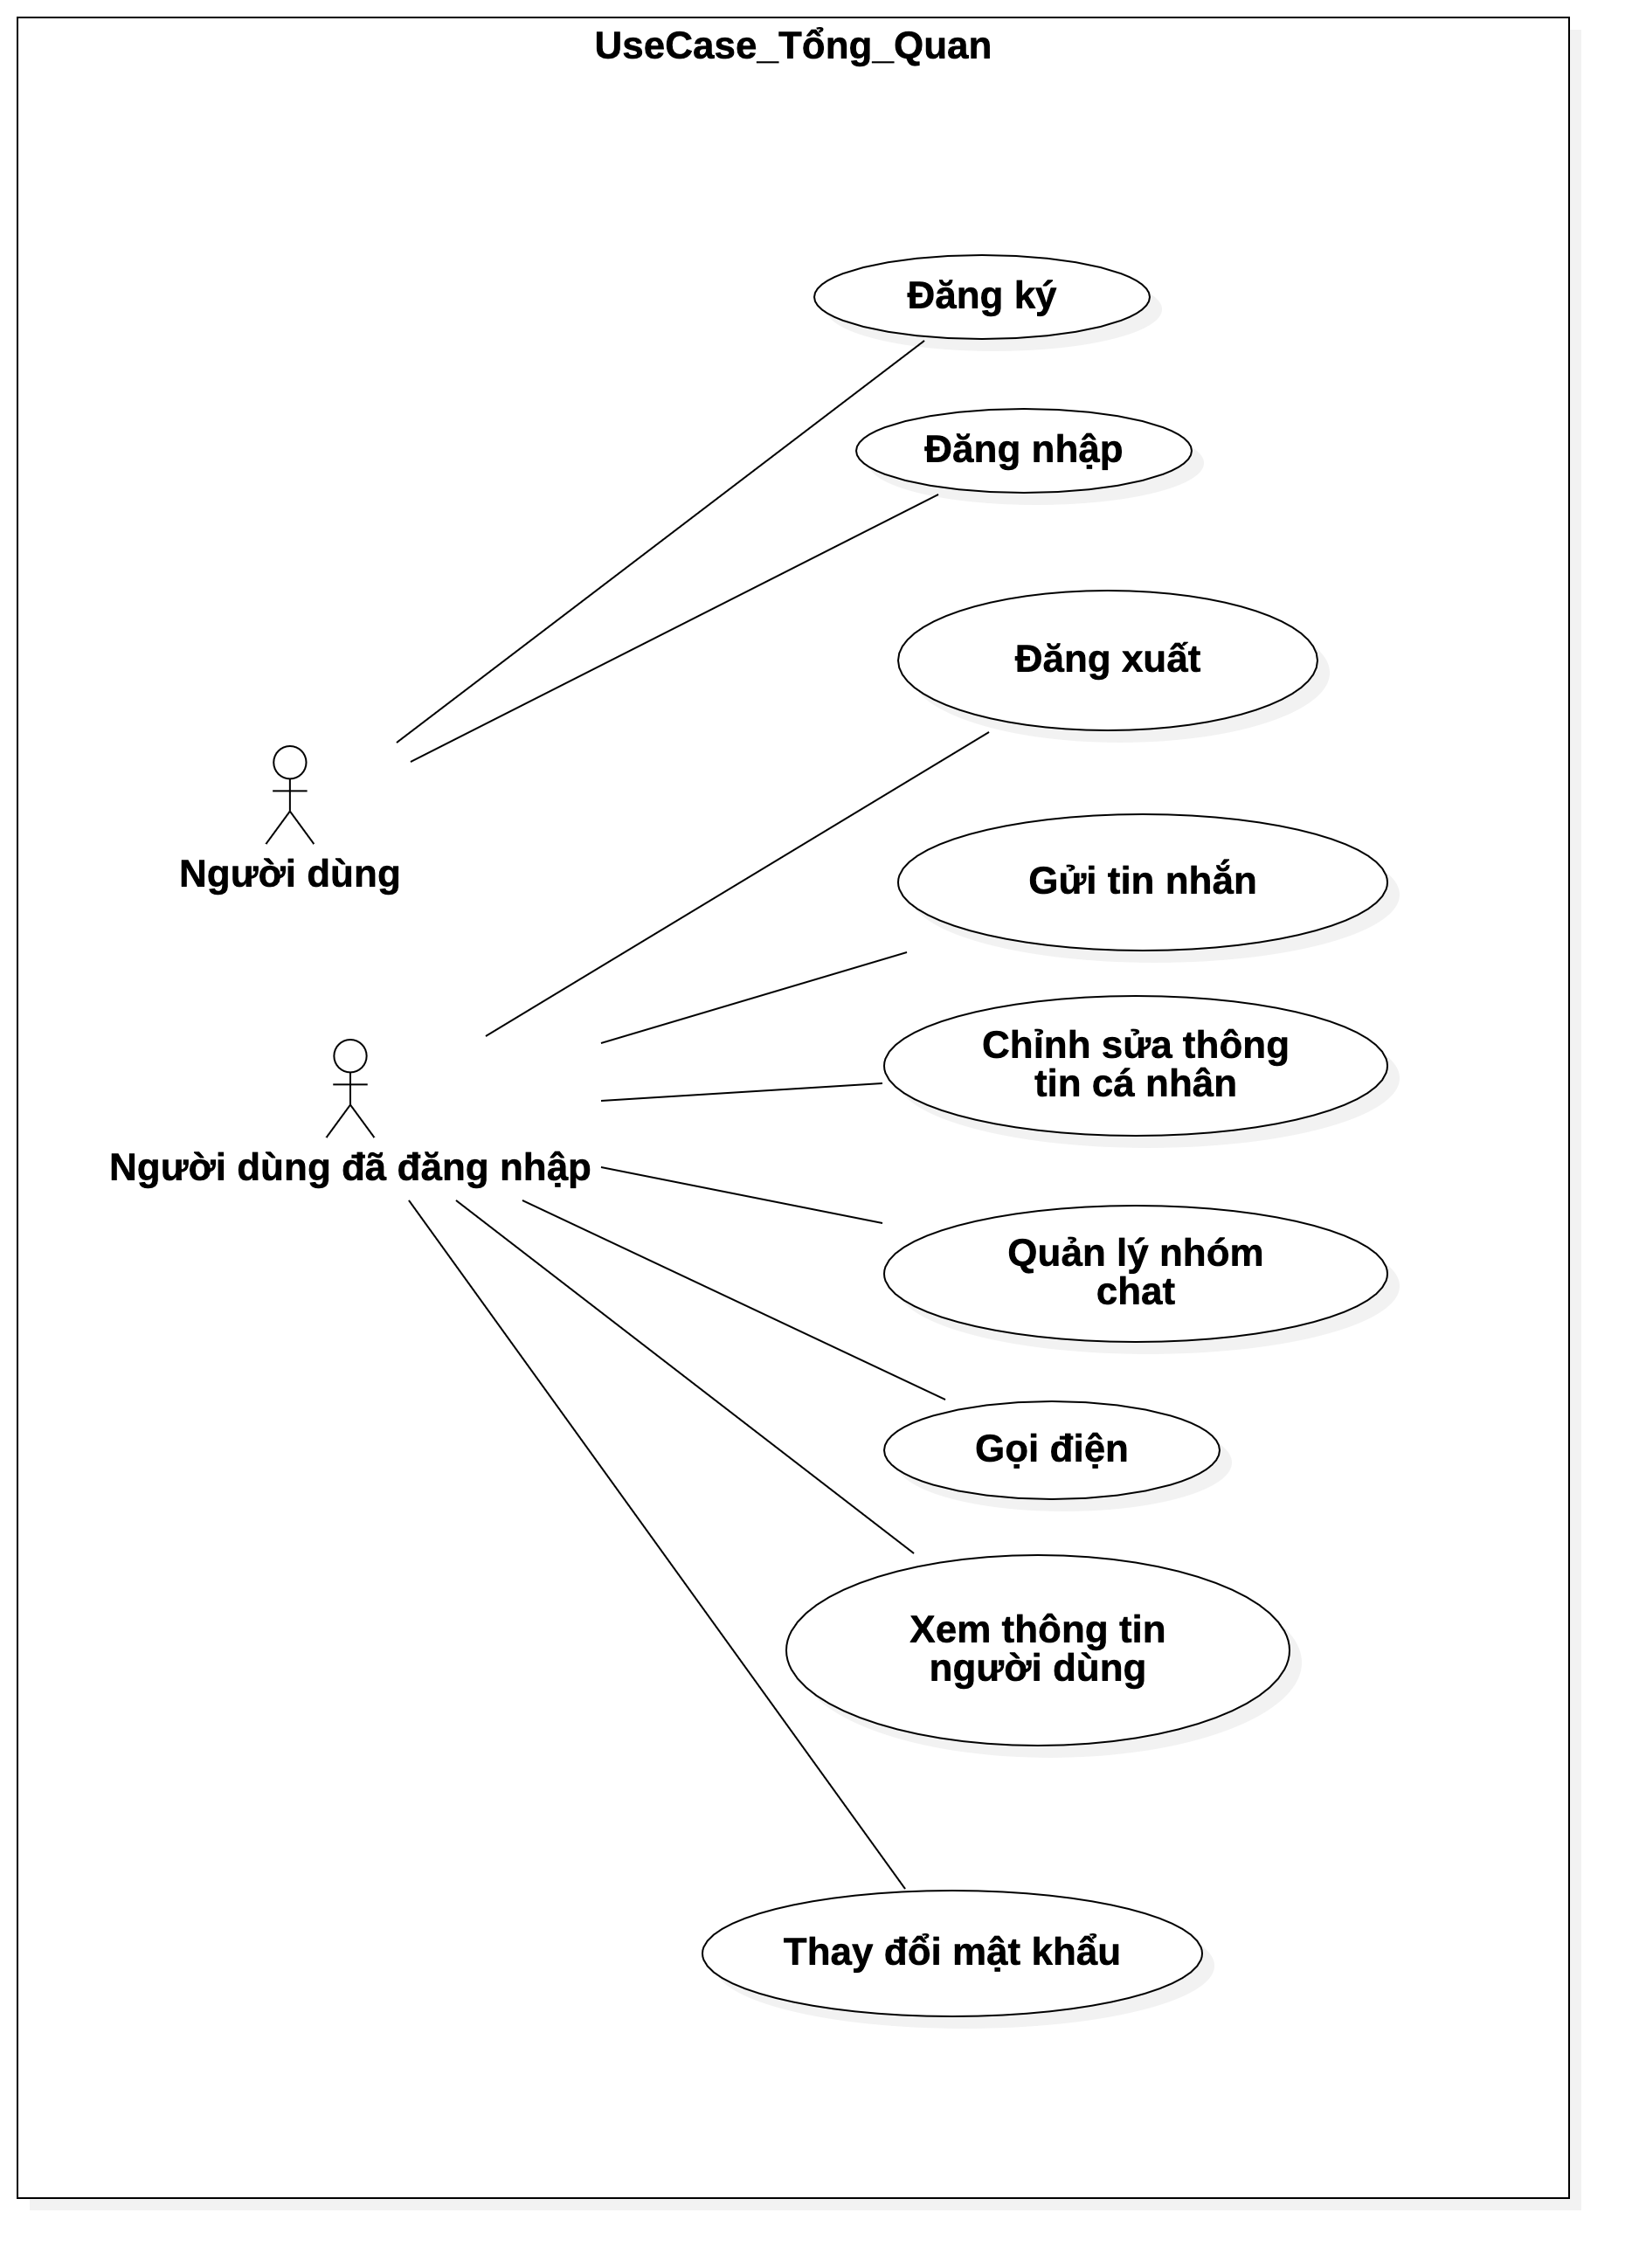
\includegraphics[width=0.9\linewidth]{Hinhve/UseCase/UseCase_Tong_Quan.png}
    \caption{Sơ đồ use case tổng quan}
    \label{fig:use_case_tổng_quan}
\end{figure}
\newpage

\subsection{Phân rã use case Nhắn tin}
\begin{figure}[H]
    \centering
    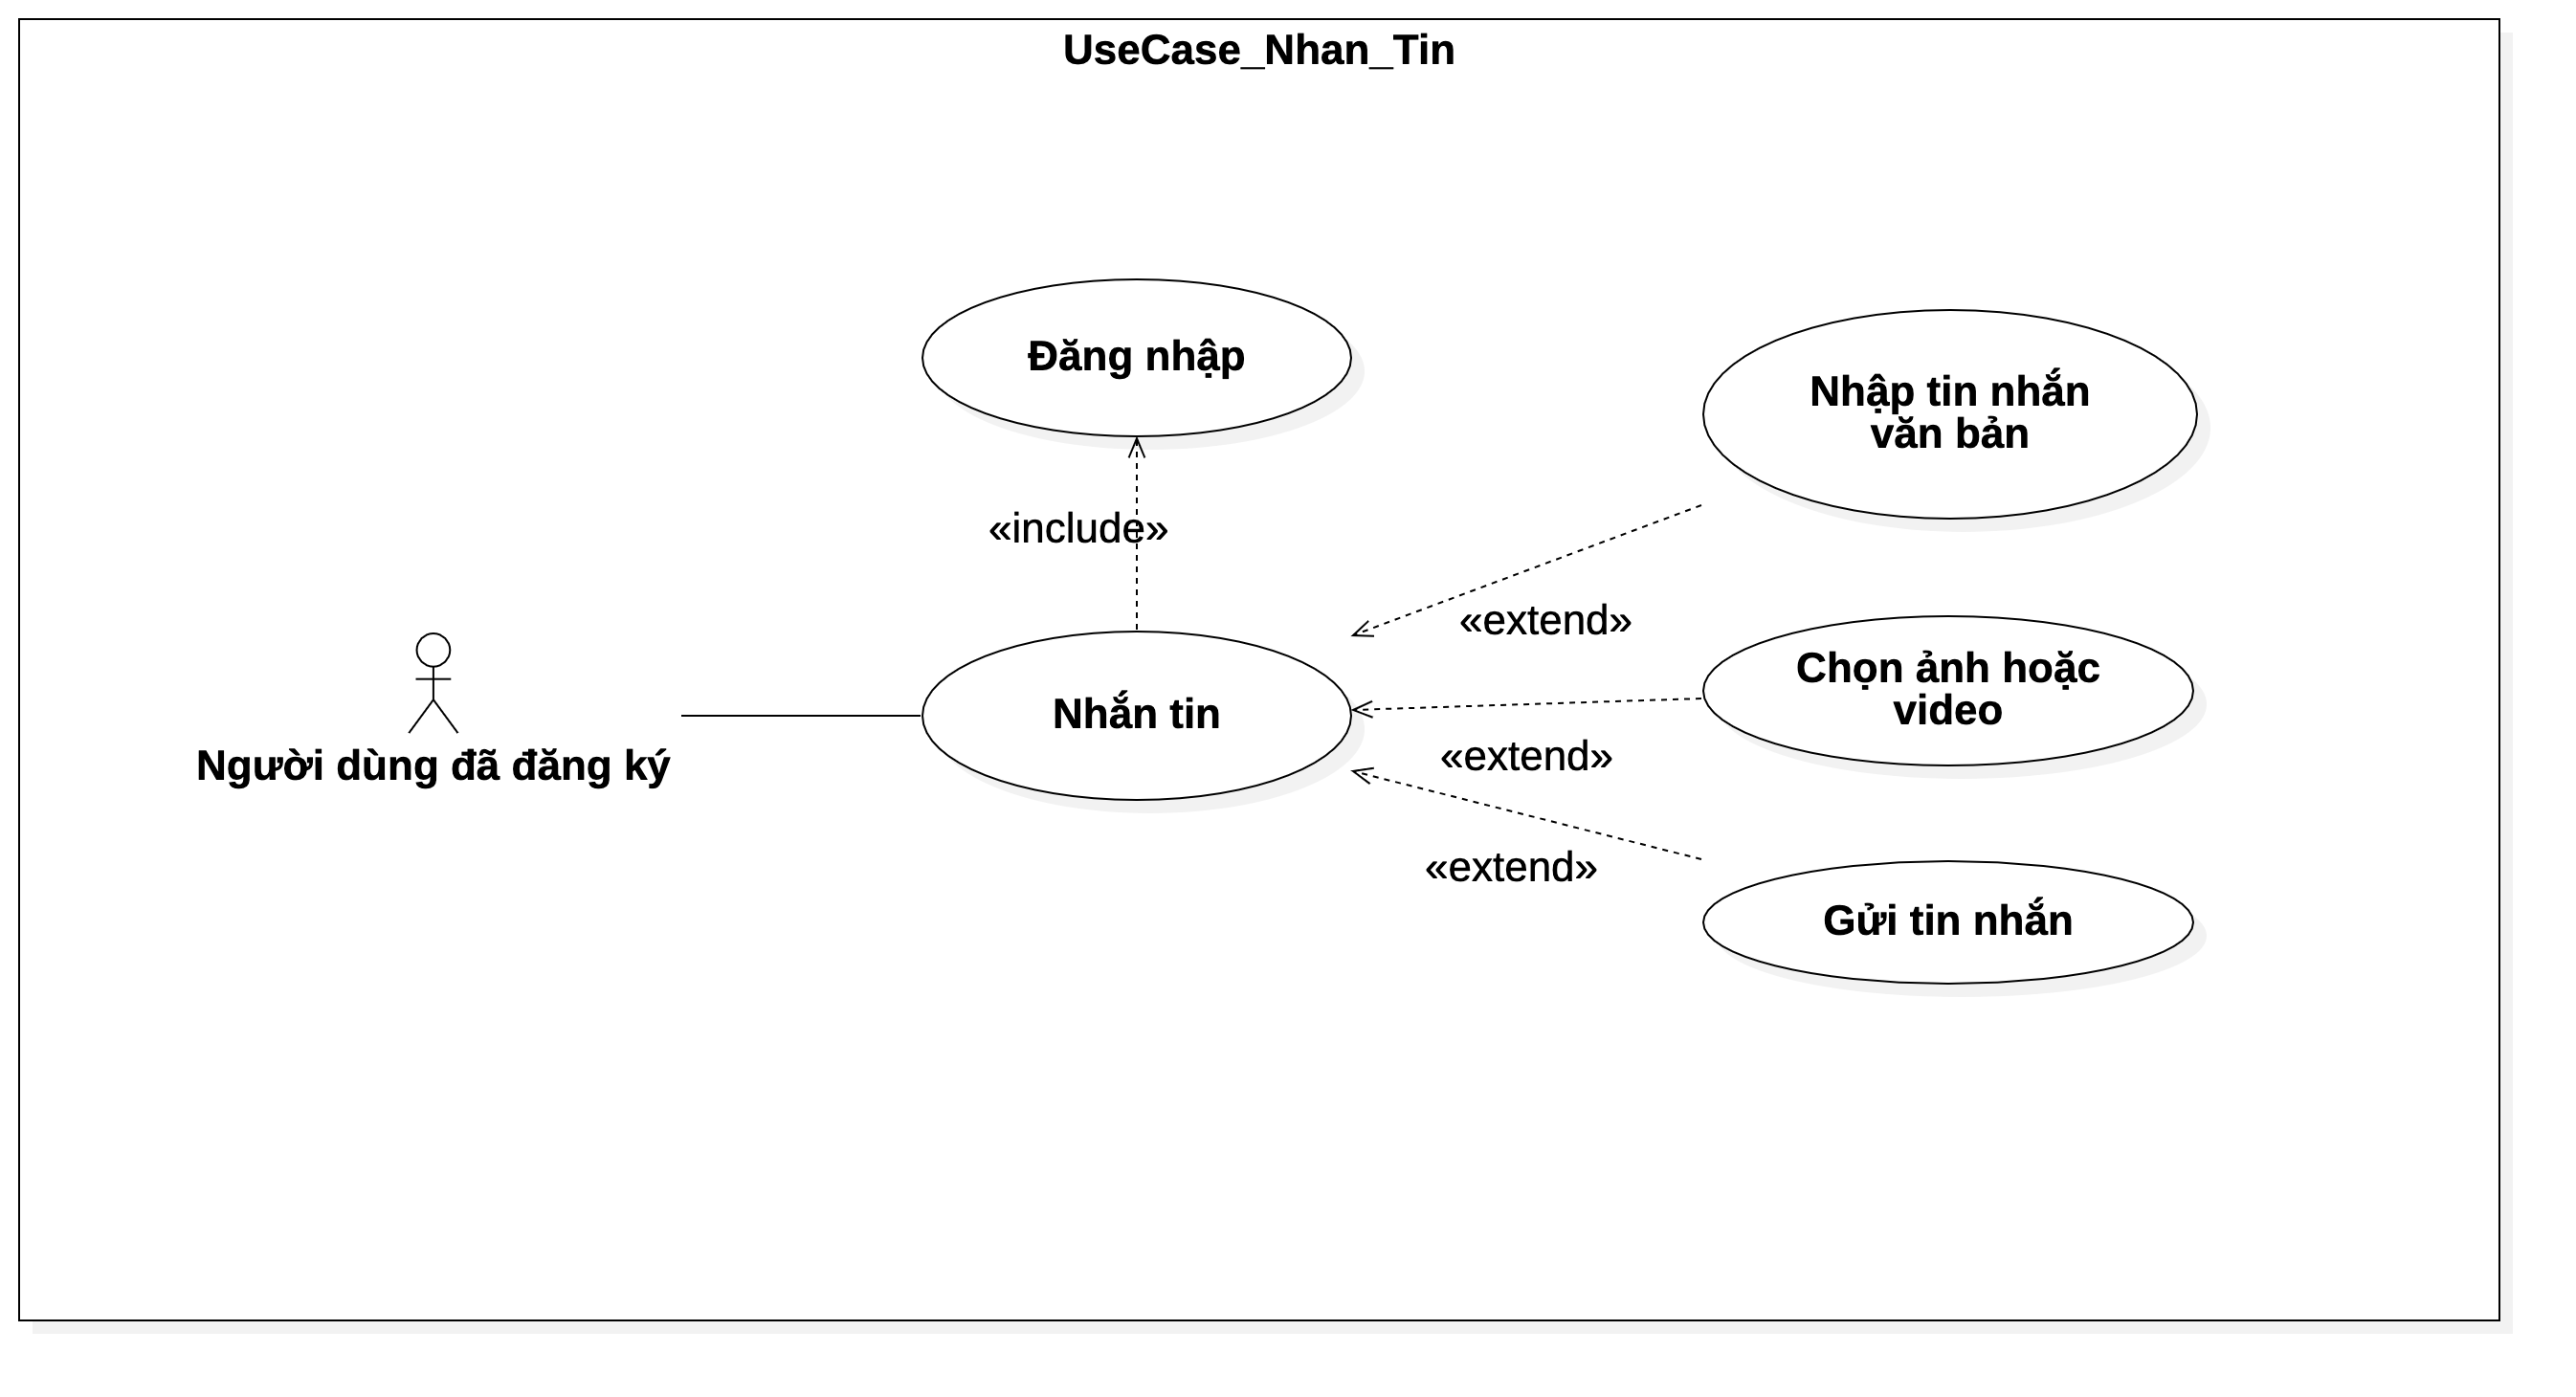
\includegraphics[width=1\linewidth]{Hinhve/UseCase/UseCase_Nhan_Tin.png}
    \caption{Phân rã use case Nhắn tin}
   \label{fig:use_case_tim_kiem}
\end{figure}

\subsection{Phân rã use case Chỉnh sửa thông tin cá nhân}
\begin{figure}[H]
    \centering
    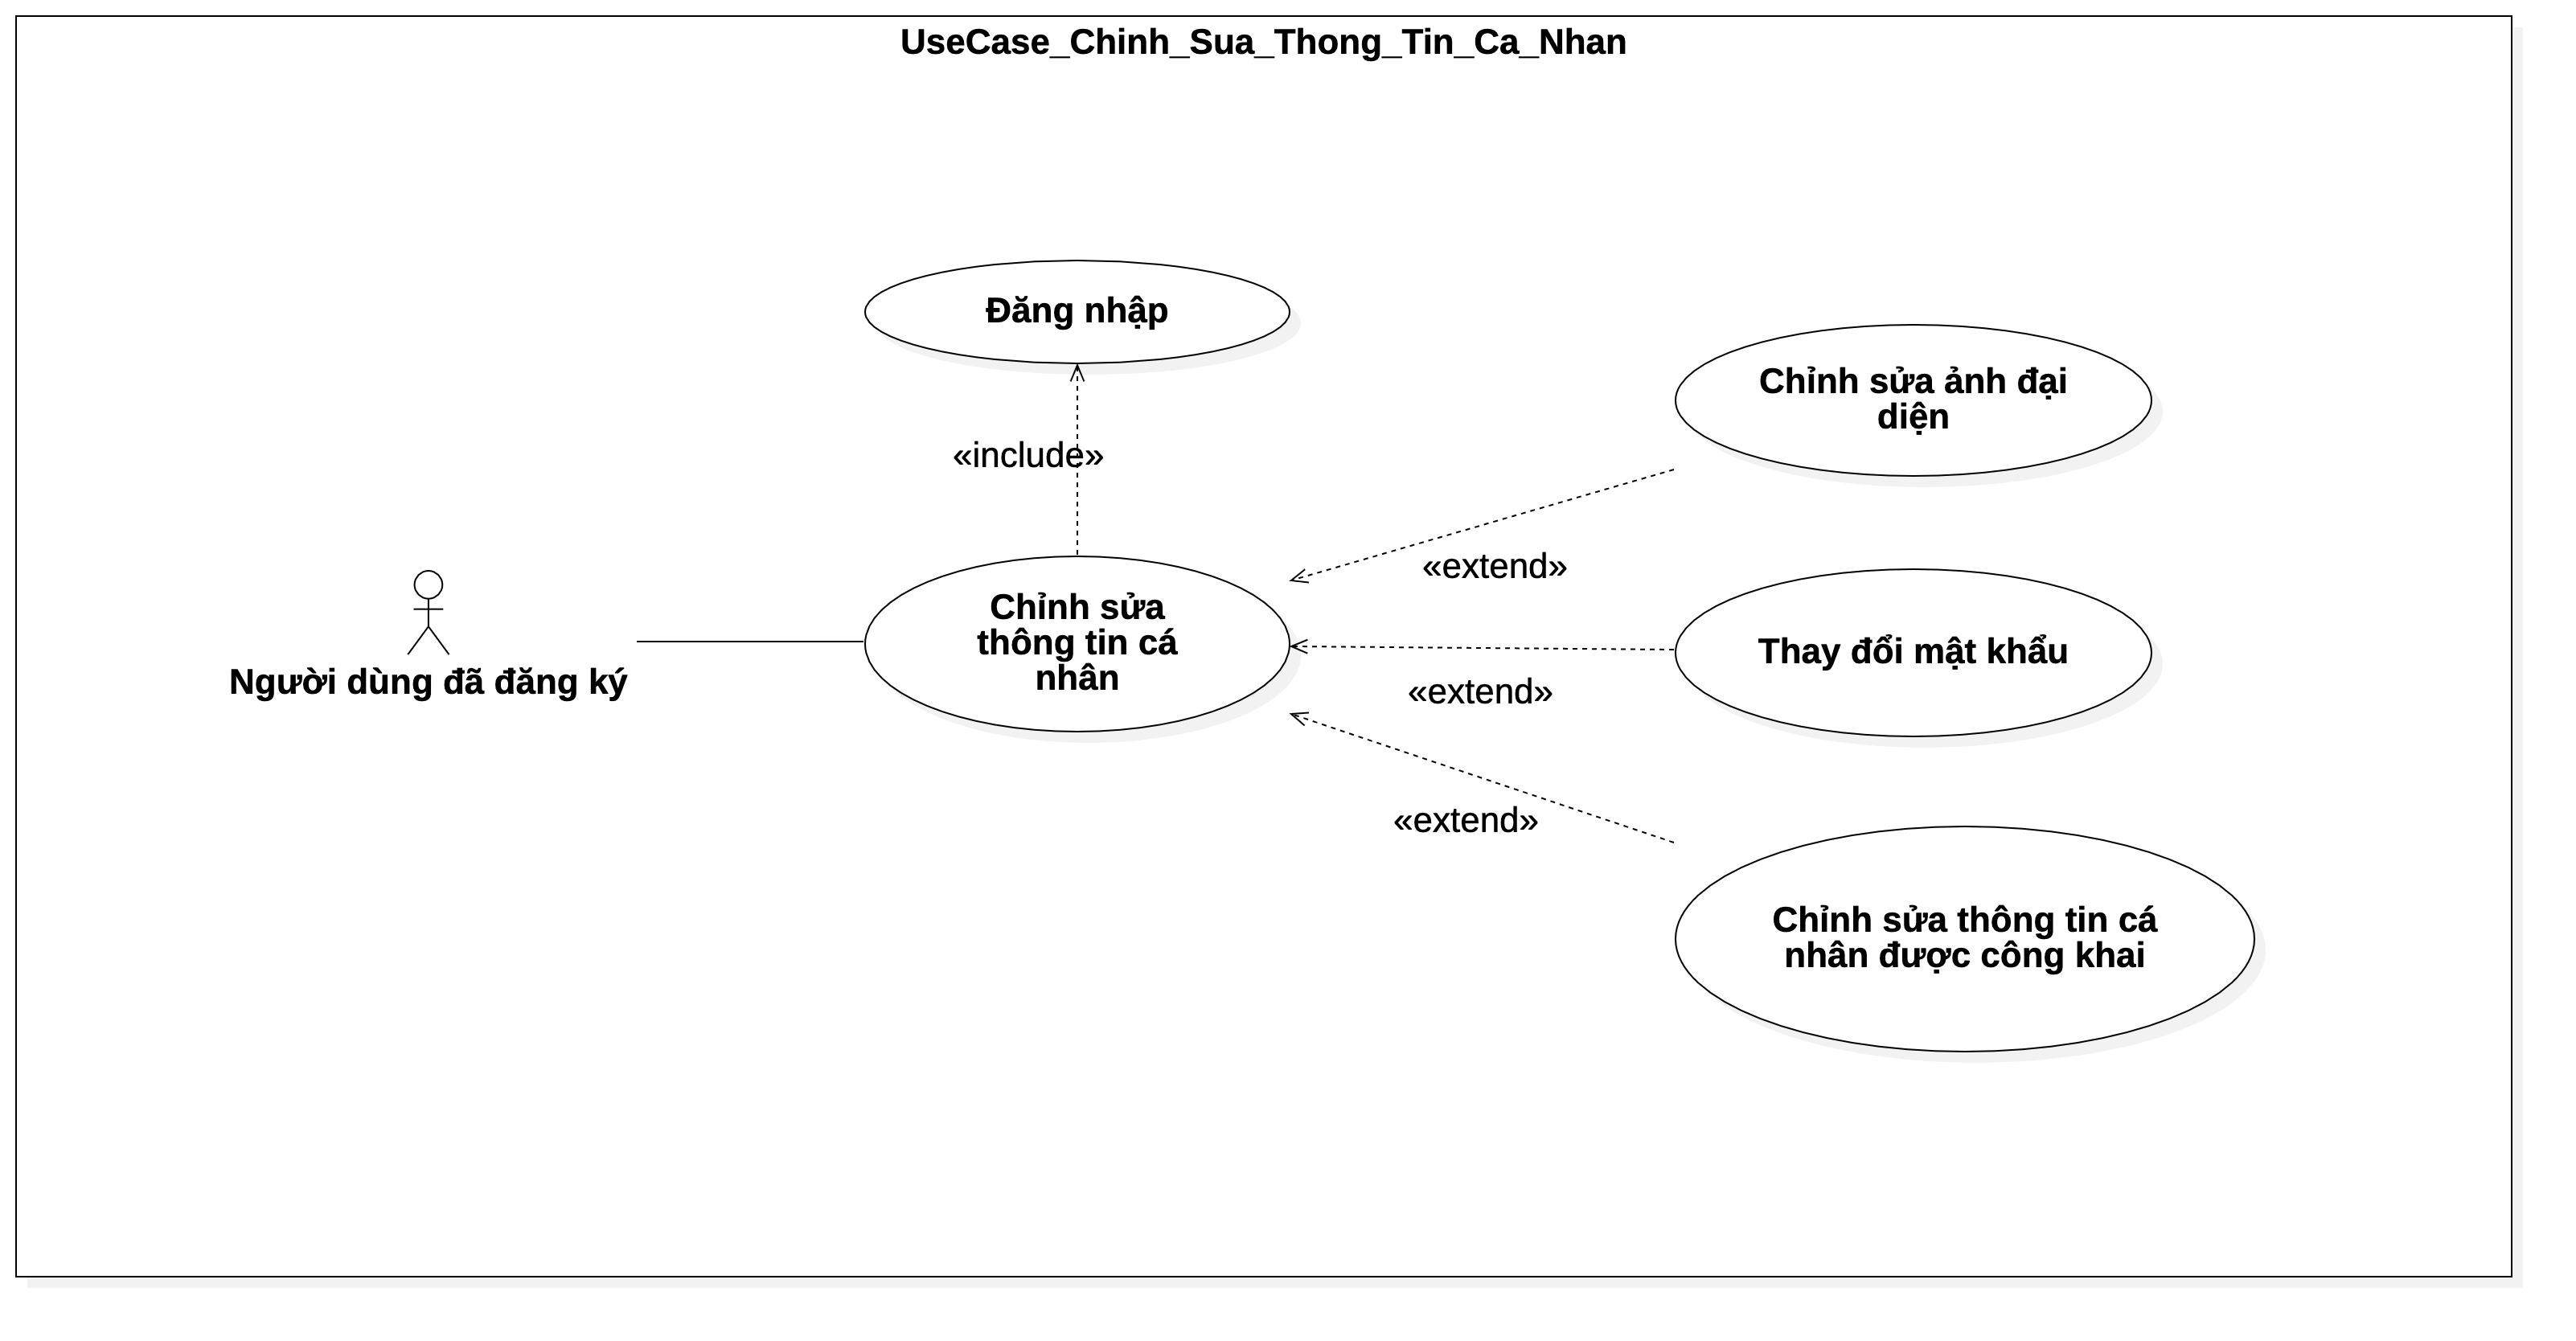
\includegraphics[width=1\linewidth]{Hinhve/UseCase/UseCase_Chinh_Sua_Thong_Tin_Ca_Nhan.png}
    \caption{Phân rã use case Chỉnh sửa thông tin cá nhân}
   \label{fig:use_case_tim_kiem}
\end{figure}

\subsection{Phân rã use case Quản lý nhóm chat}
\begin{figure}[H]
    \centering
    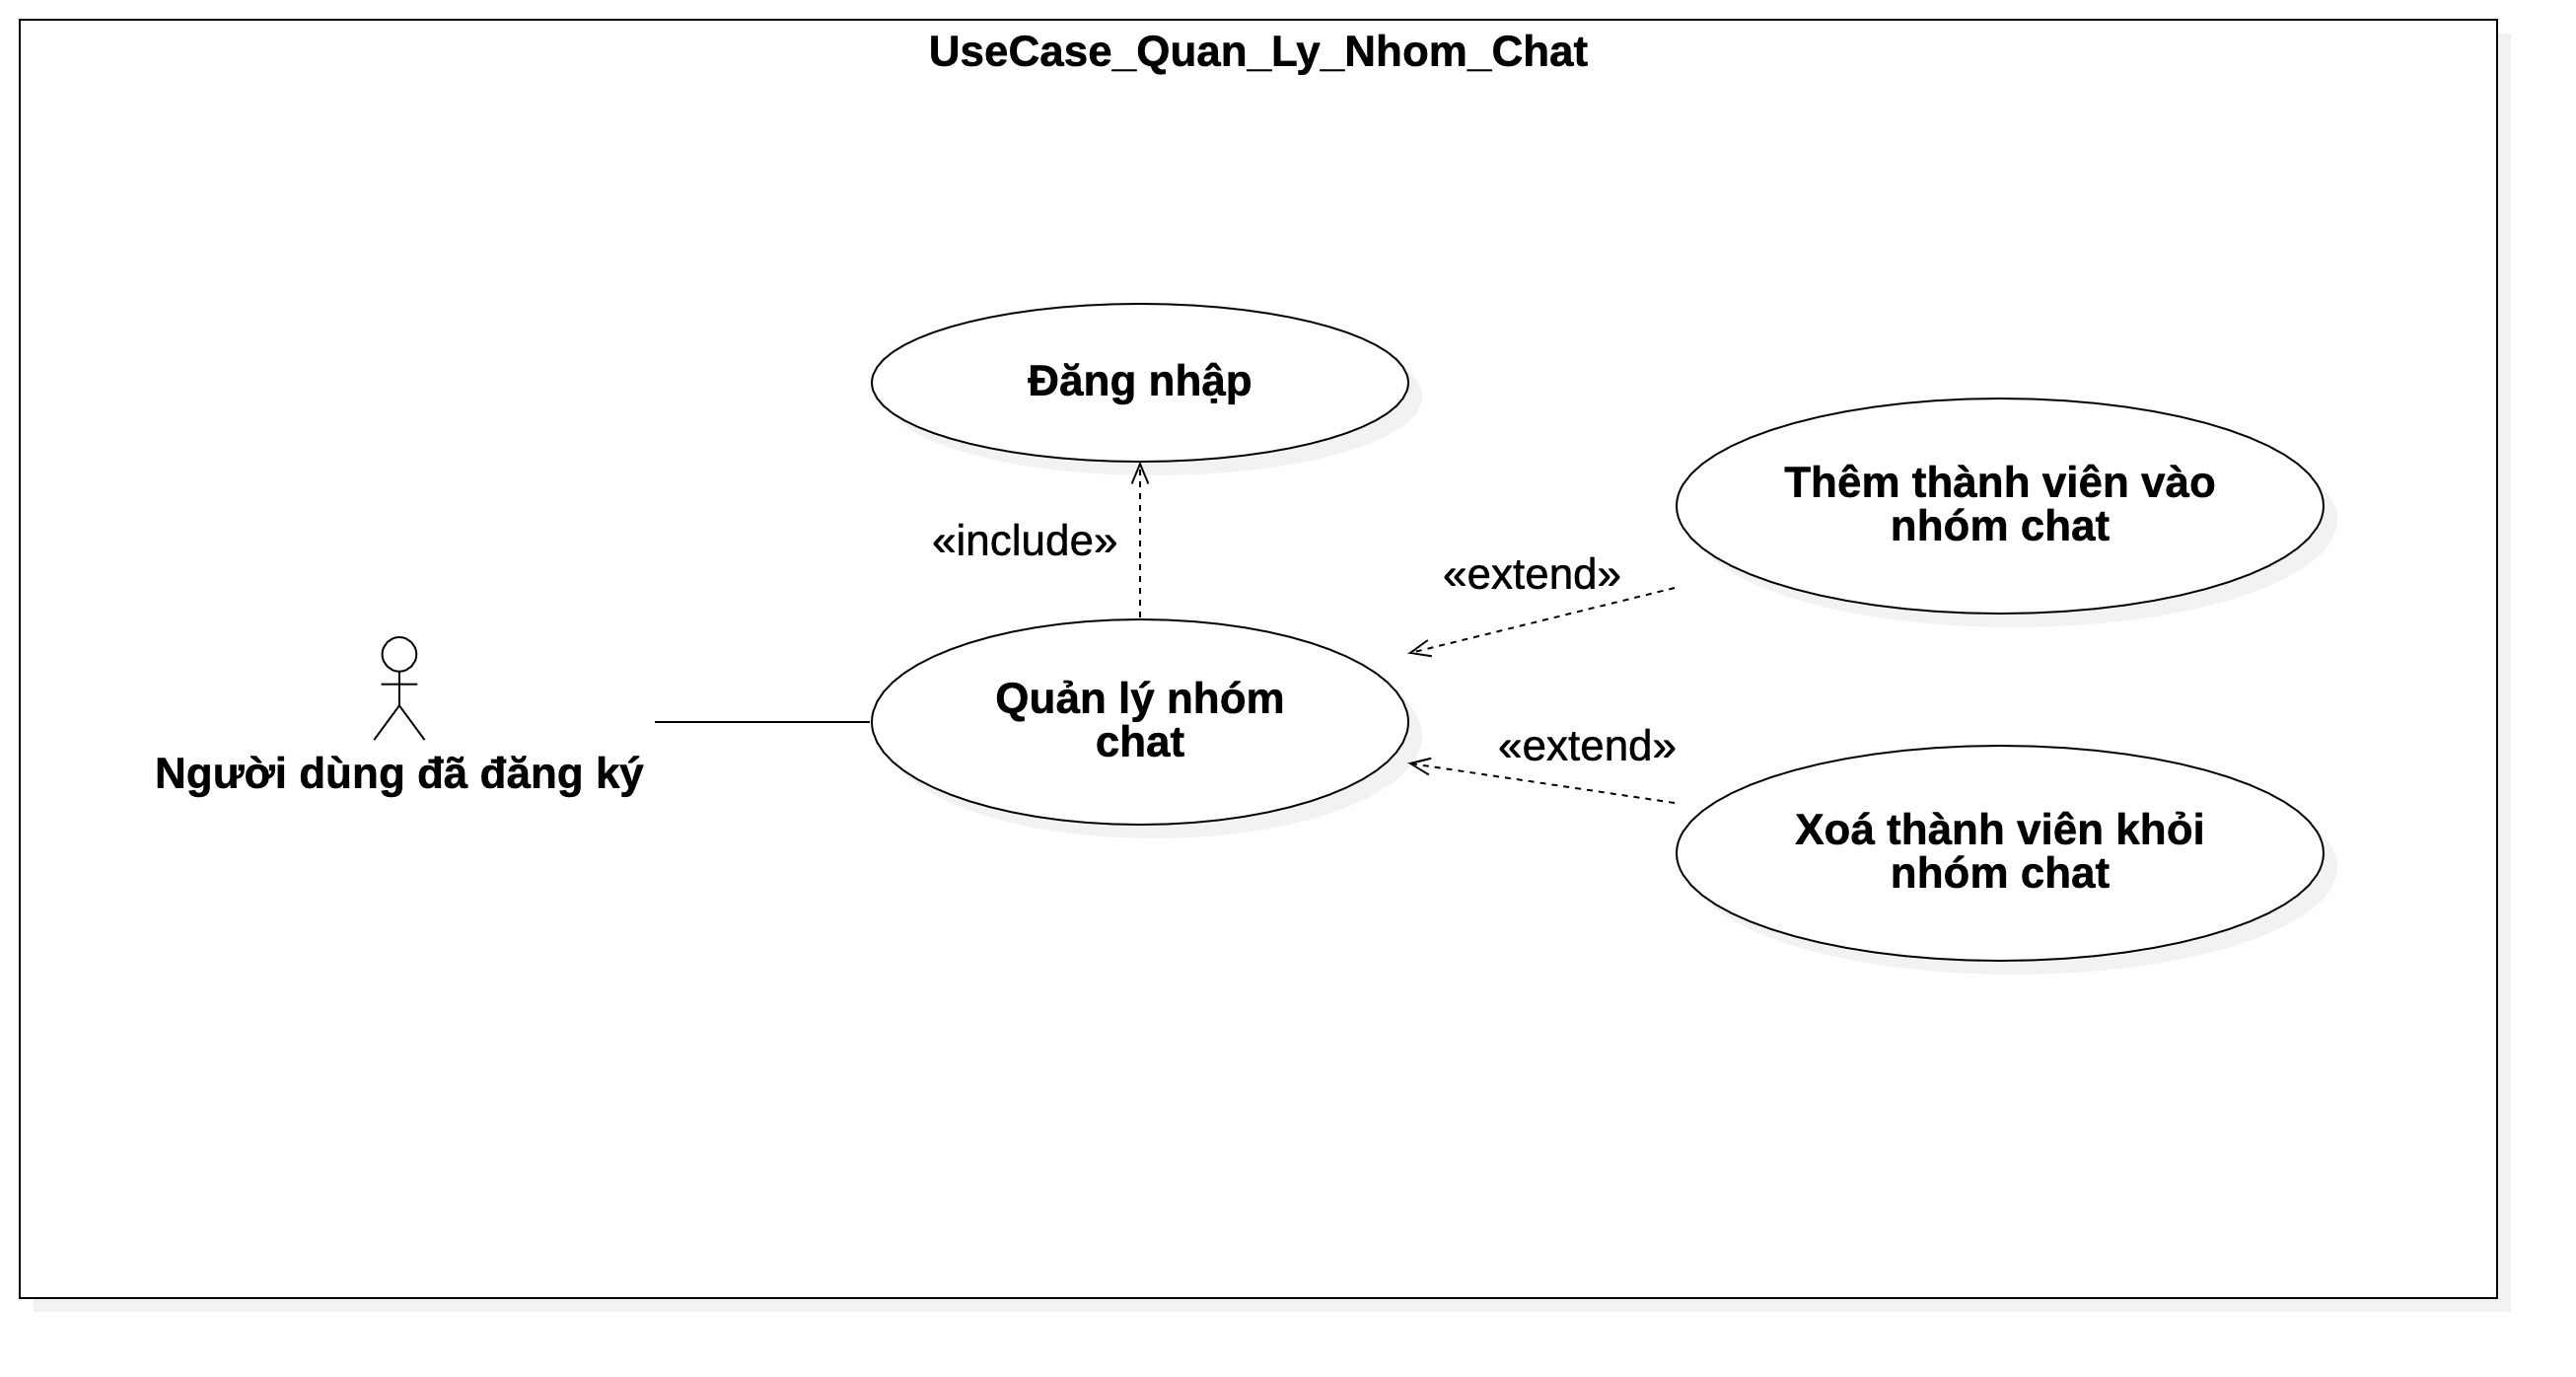
\includegraphics[width=1\linewidth]{Hinhve/UseCase/UseCase_Quan_Ly_Nhom_Chat.png}
    \caption{Phân rã use case Quản lý nhóm chat}
    \label{fig:use_case_binh_luan_task}
\end{figure}     



\section{Quy trình nghiệp vụ}
\label{subsection:2.3}

\subsection{Nghiệp vụ Đăng ký}
\begin{figure}[H]
   \centering
    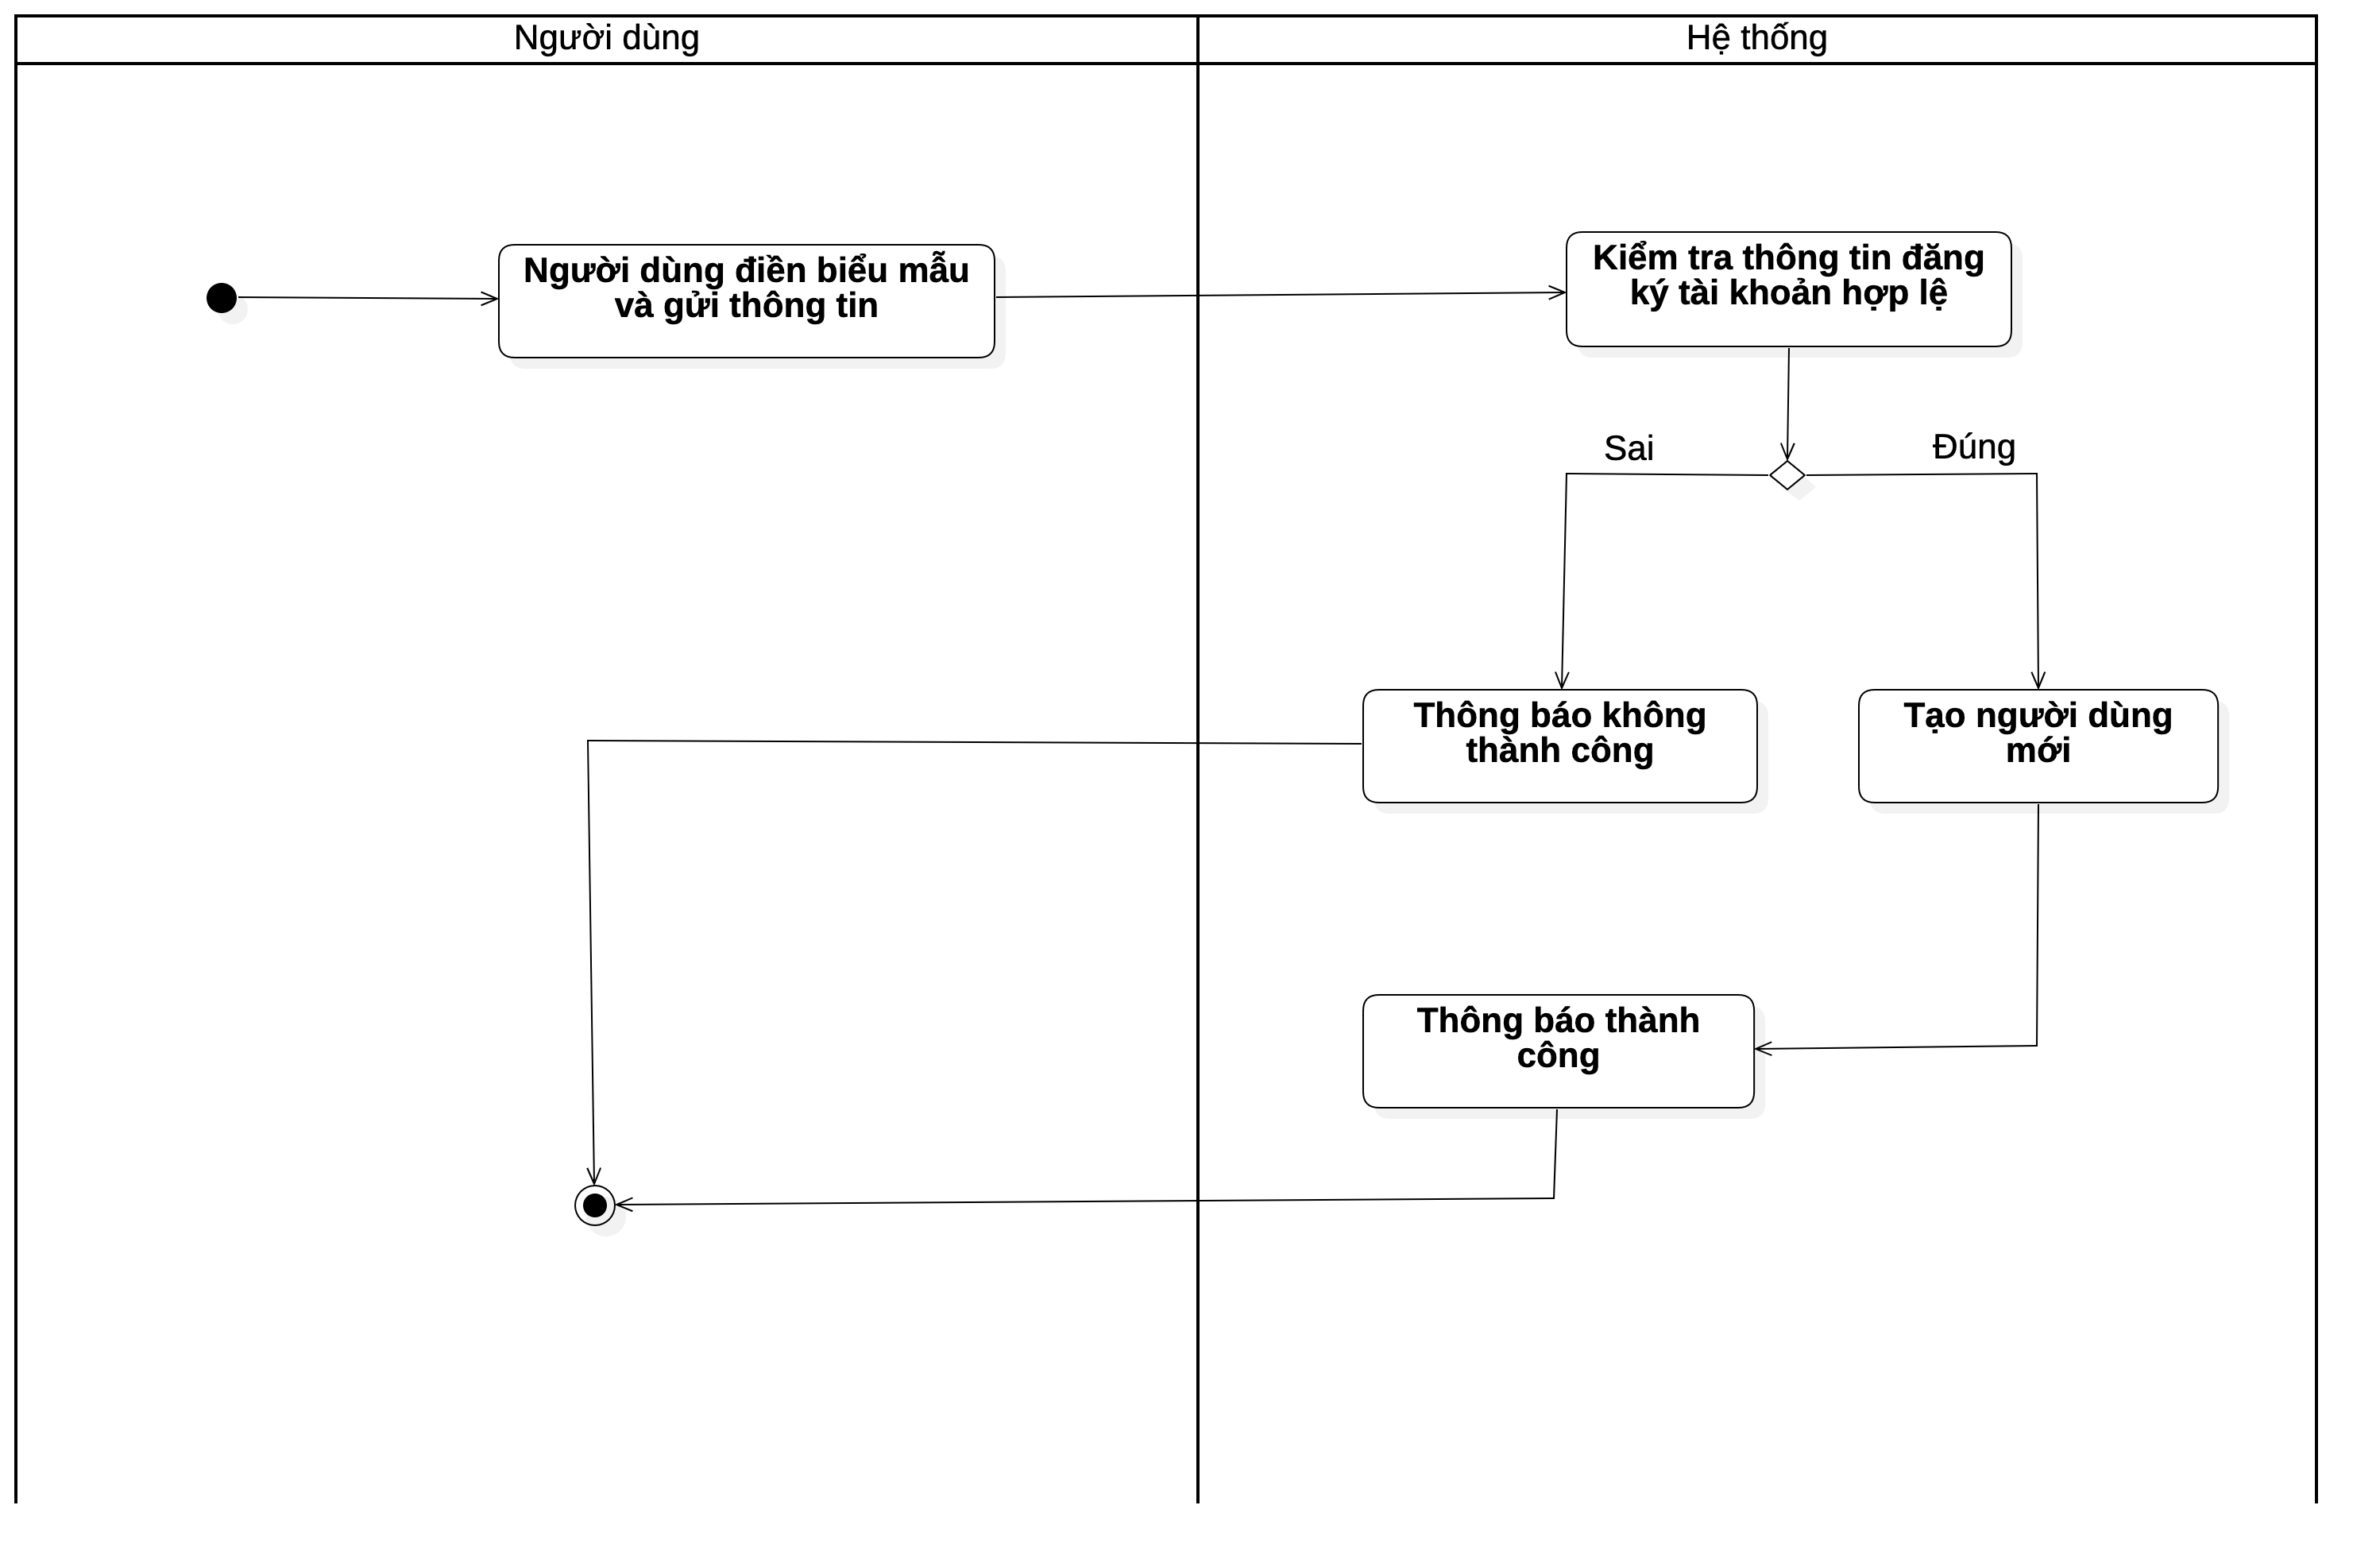
\includegraphics[width=1\linewidth]{Hinhve/Activity/Activity_Dang_Ky.png}
    \caption{Sơ đồ hoạt động quy trình nghiệp vụ Đăng ký}
    \label{fig:dang_nhap}
\end{figure}

\subsection{Nghiệp vụ Đăng nhập}
\begin{figure}[H]
   \centering
    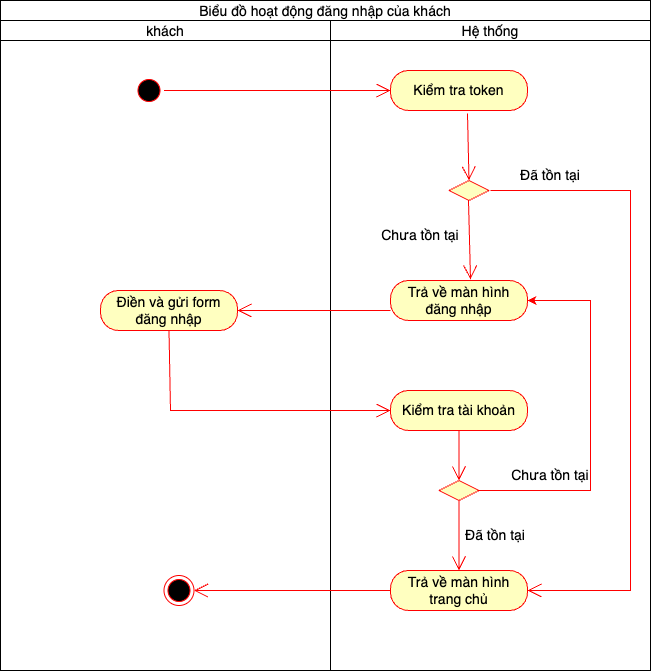
\includegraphics[width=1\linewidth]{Hinhve/Activity/dang_nhap.png}
    \caption{Sơ đồ hoạt động quy trình nghiệp vụ Đăng nhập}
    \label{fig:dang_nhap}
\end{figure}
\hfill

\subsection{Nghiệp vụ Thay đổi mật khẩu}
\begin{figure}[H]
   \centering
    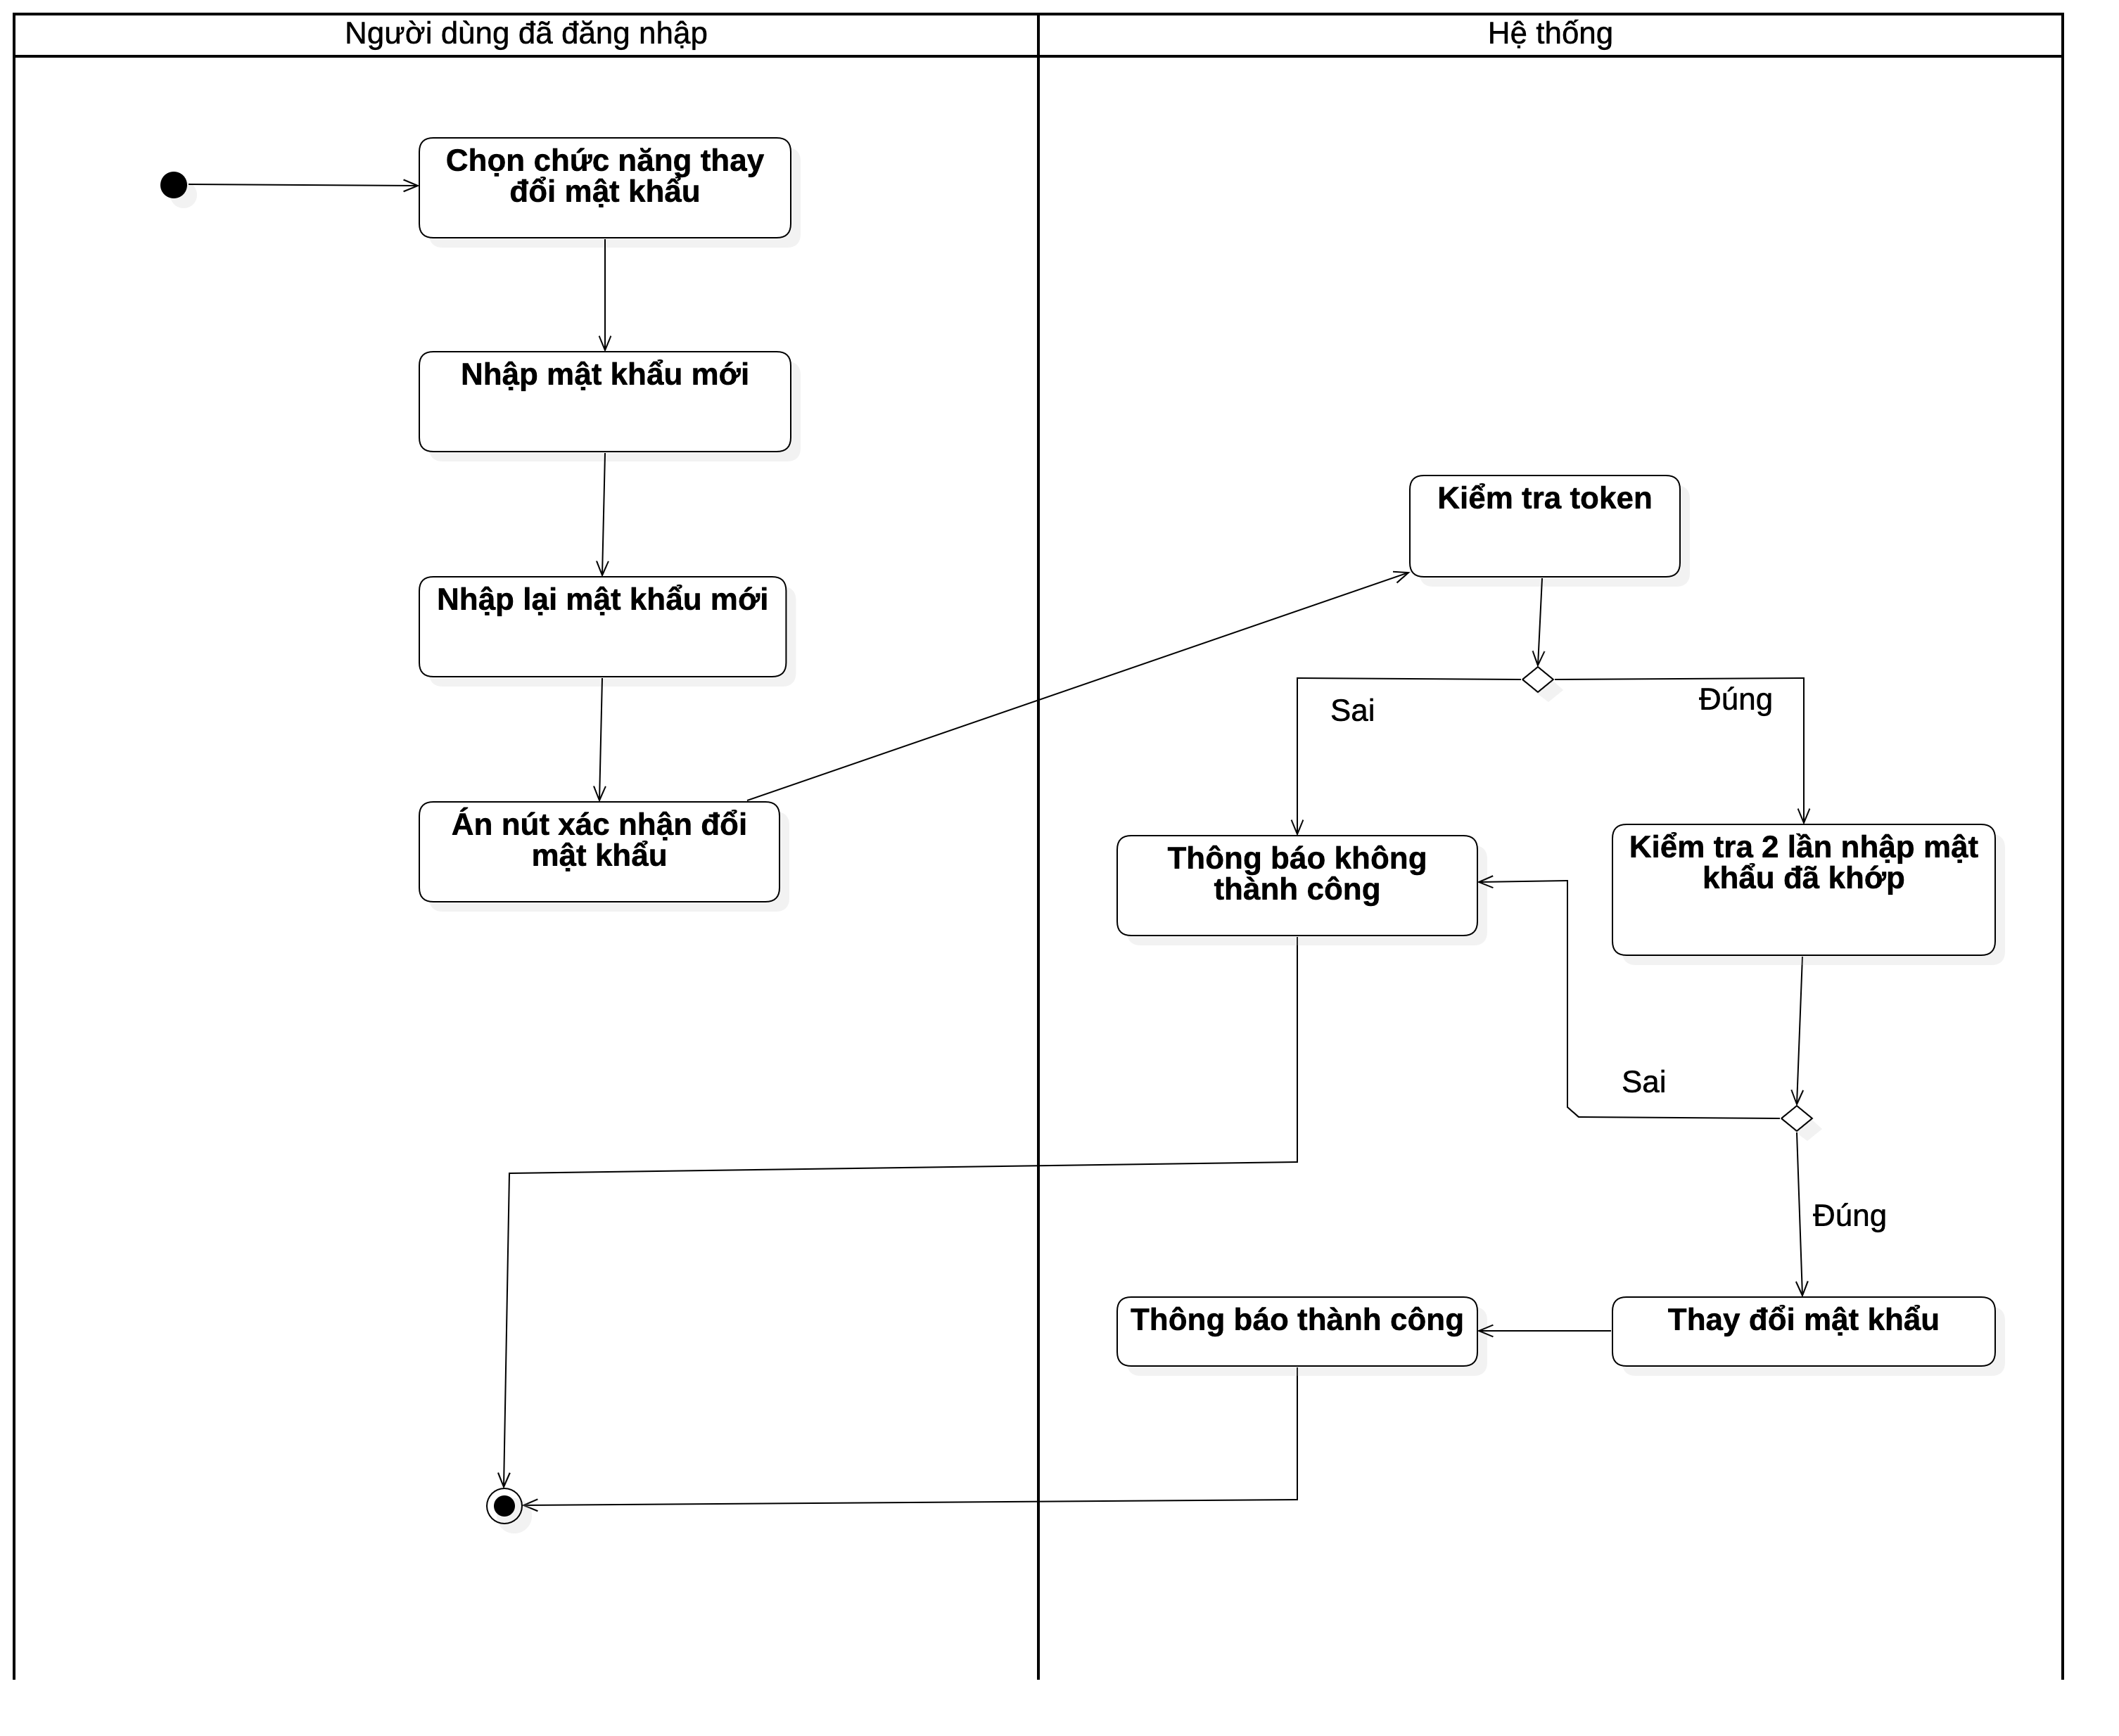
\includegraphics[width=1\linewidth]{Hinhve/Activity/Activity_Thay_Doi_Mat_Khau.png}
    \caption{Sơ đồ hoạt động quy trình nghiệp vụ Thay đổi mật khẩu}
    \label{fig:dang_nhap}
\end{figure}
\hfill

\subsection{Nghiệp vụ Chỉnh sửa thông tin cá nhân được công khai}
\begin{figure}[H]
   \centering
    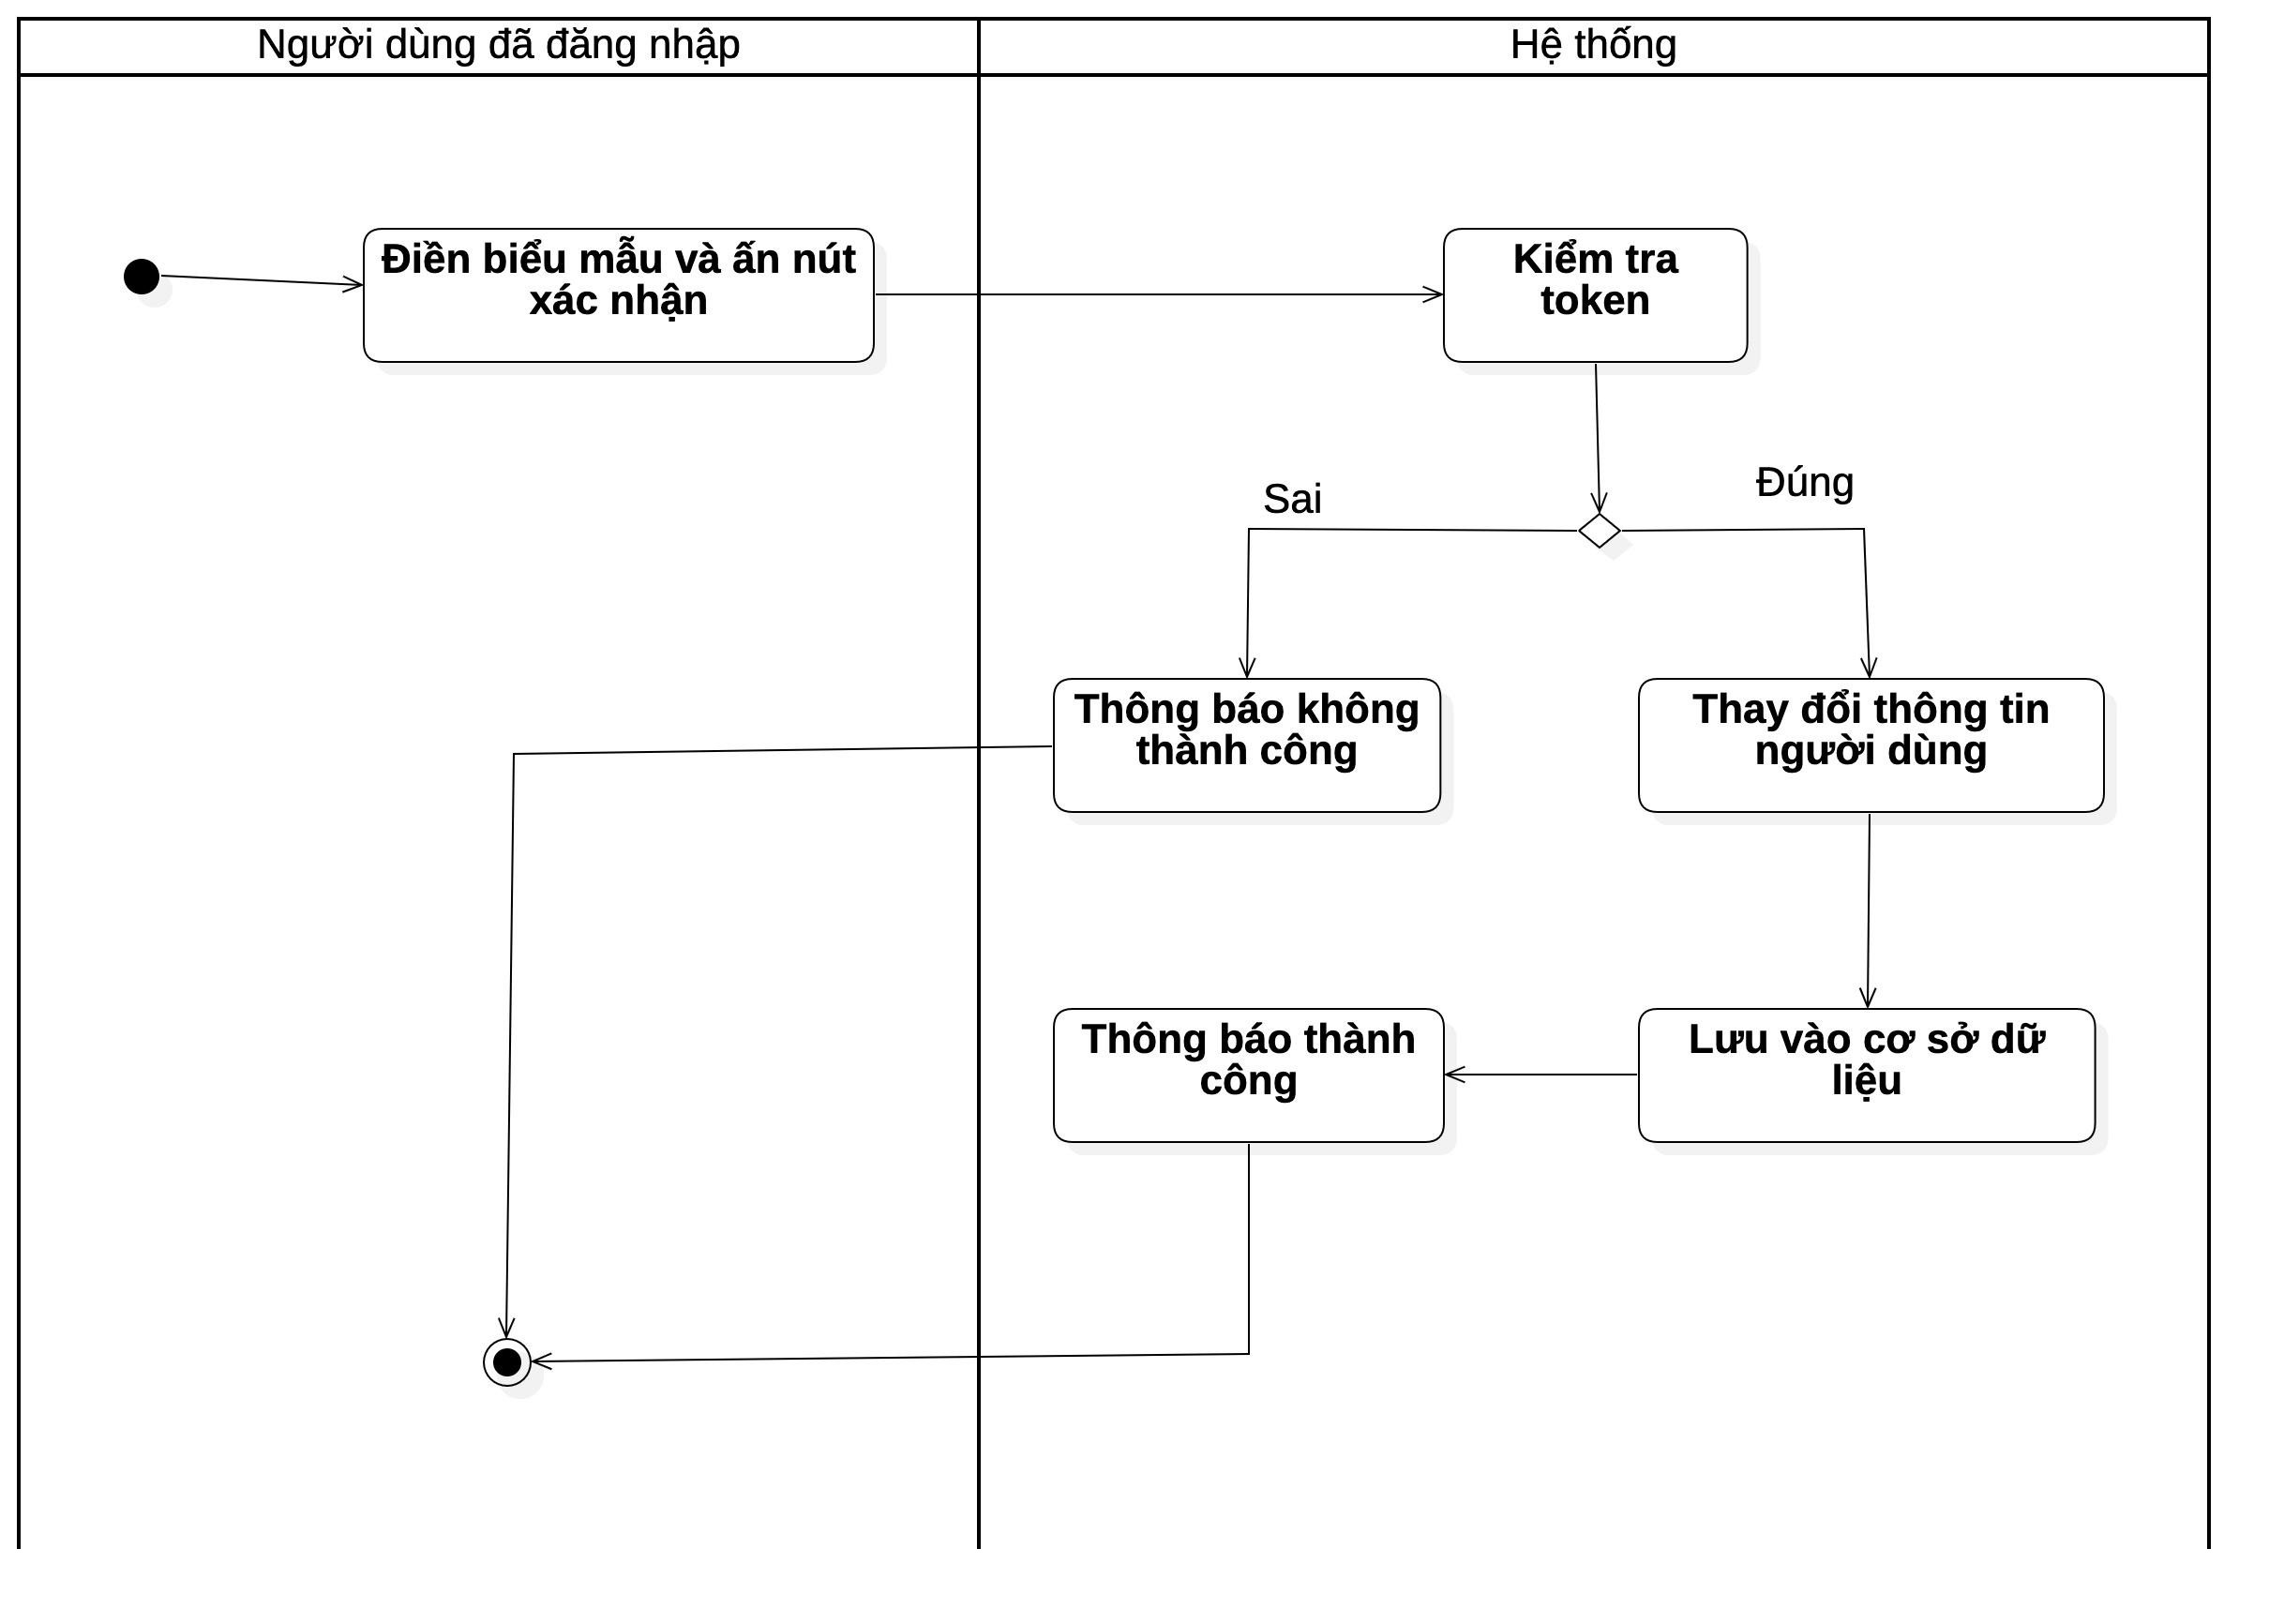
\includegraphics[width=0.9\linewidth]{Hinhve/Activity/Activity_Chinh_Sua_Thong_Tin_Ca_Nhan_Duoc_Cong_Khai.png}
    \caption{Sơ đồ hoạt động quy trình nghiệp vụ Chỉnh sửa thông tin cá nhân được công khai}
    \label{fig:dang_nhap}
\end{figure}

\subsection{Nghiệp vụ Thêm thành viên vào nhóm}
\begin{figure}[H]
   \centering
    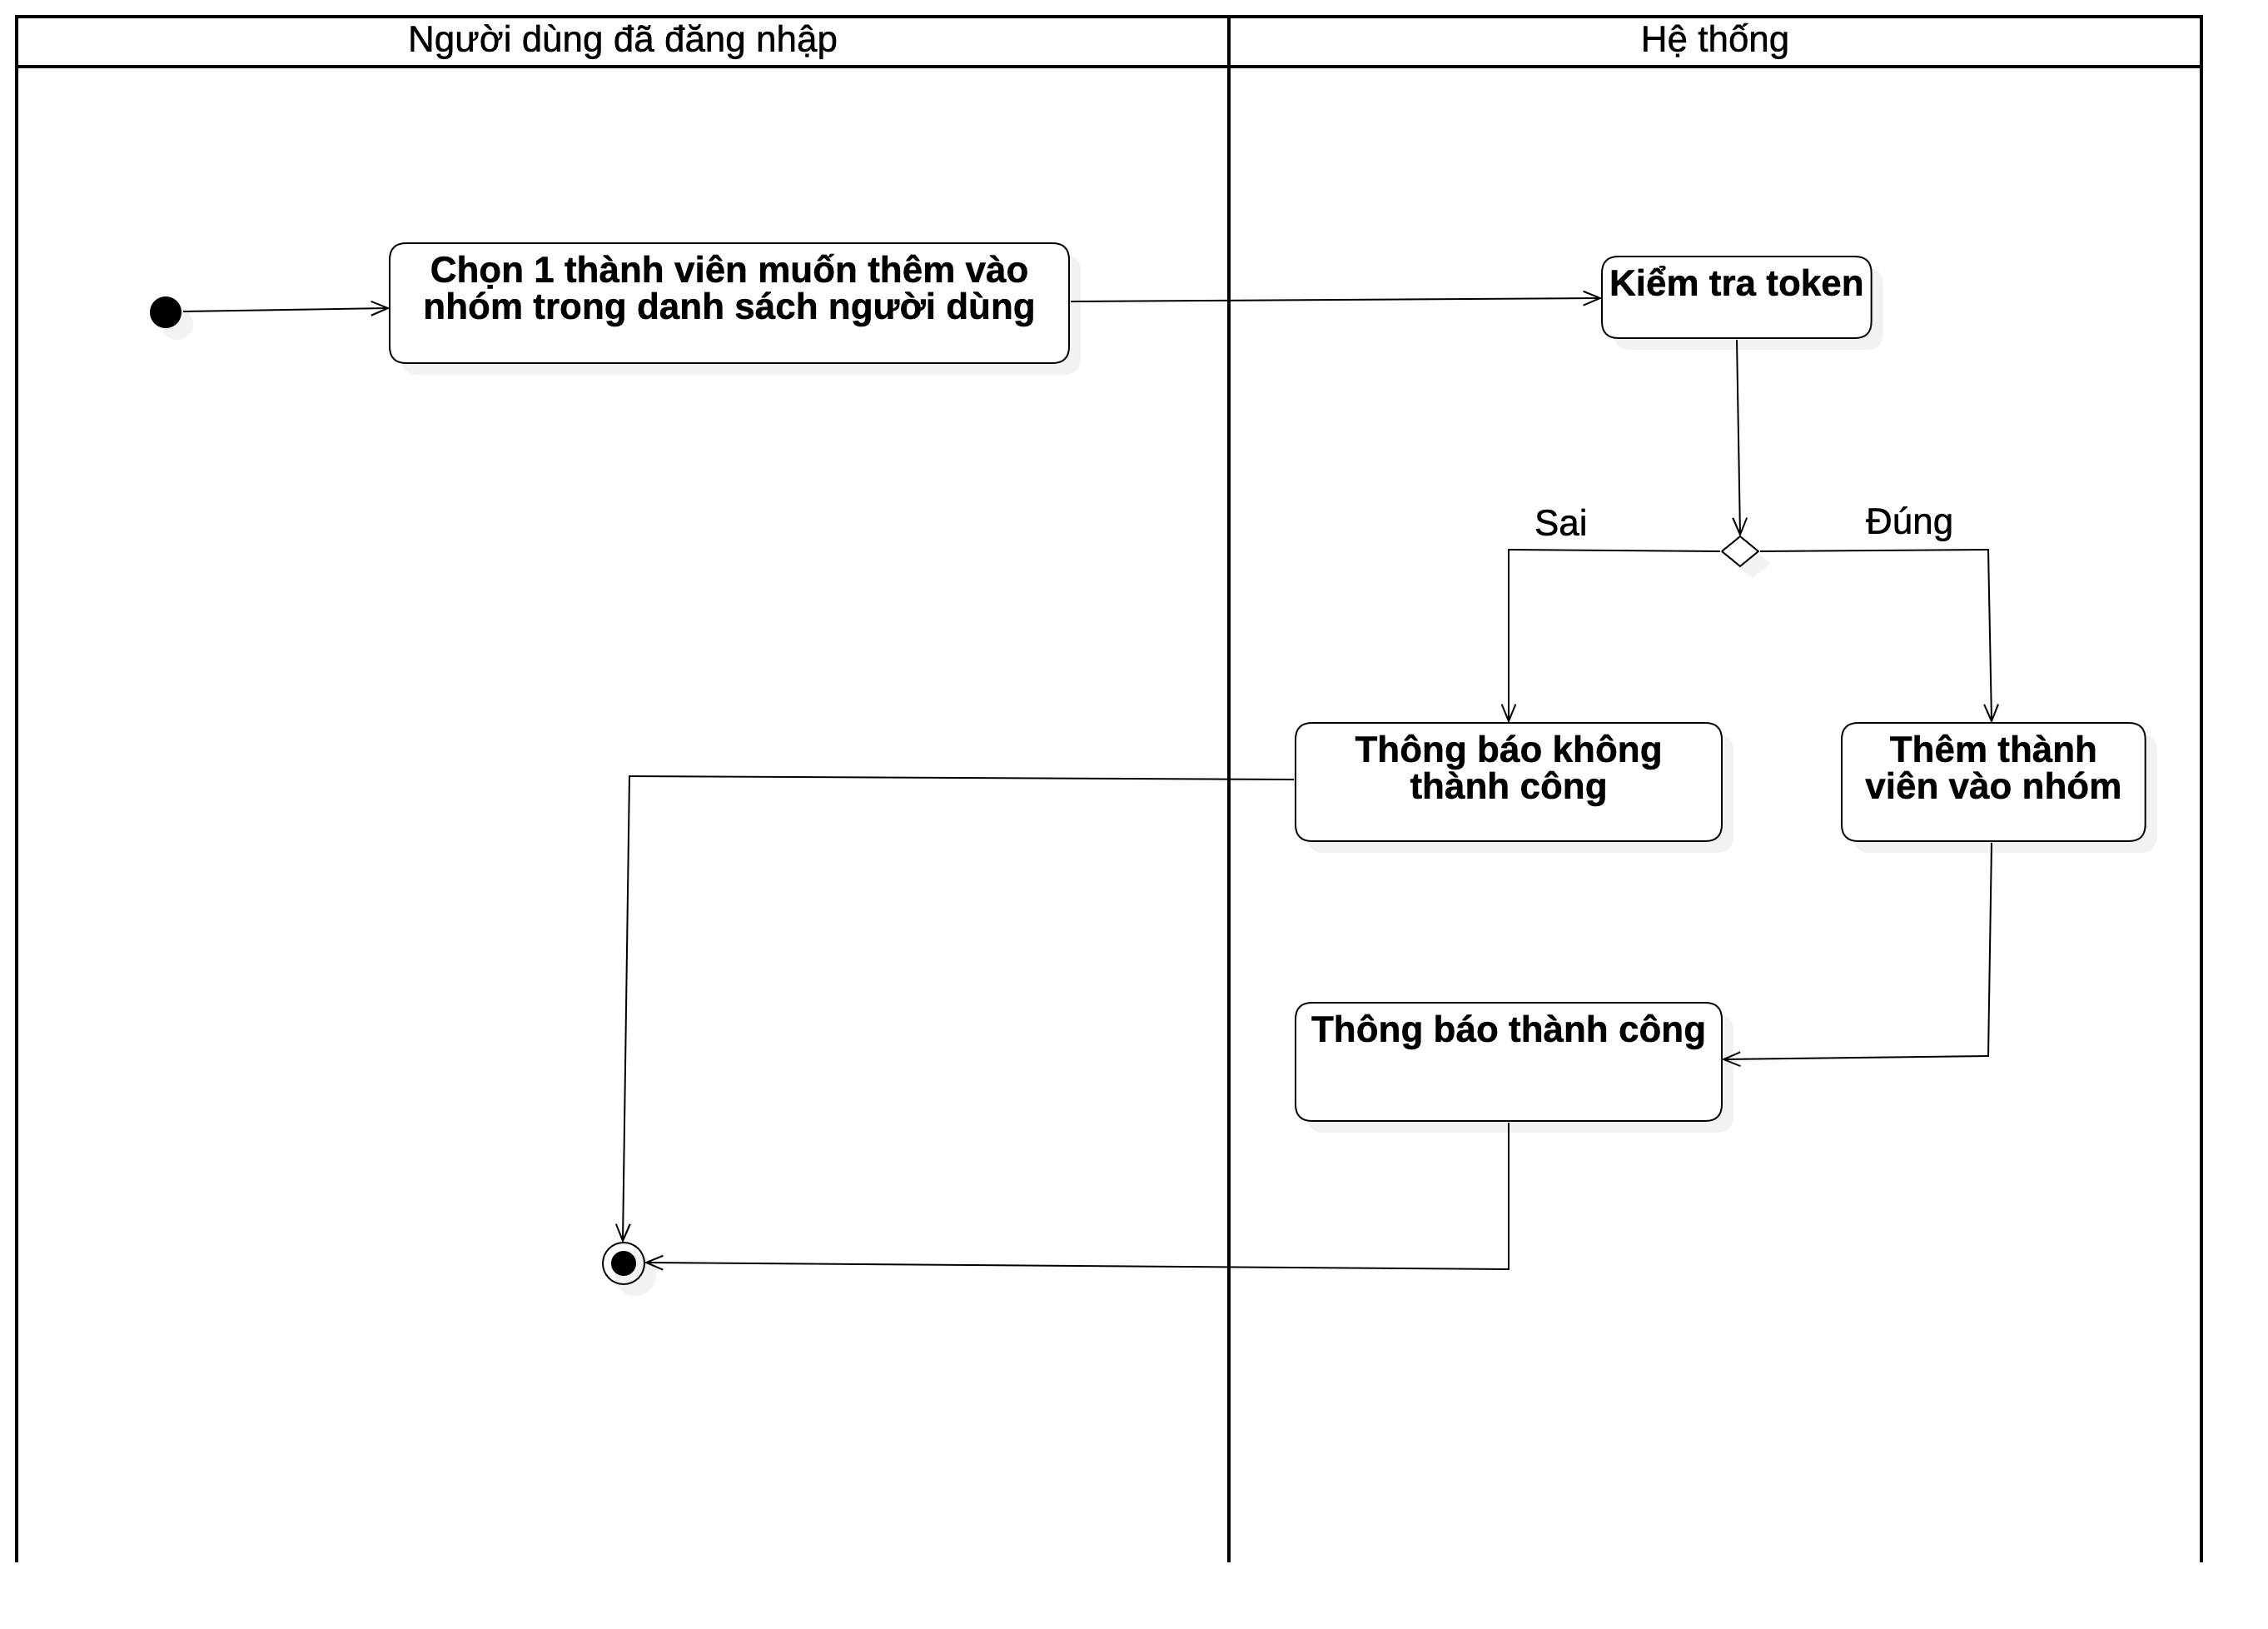
\includegraphics[width=0.9\linewidth]{Hinhve/Activity/Activity_Them_Thanh_Vien_Vao_Nhom_Chat.png}
    \caption{Sơ đồ hoạt động quy trình nghiệp vụ Thêm thành viên vào nhóm}
    \label{fig:dang_nhap}
\end{figure}

\subsection{Nghiệp vụ Xoá thành viên khỏi nhóm chat}
\begin{figure}[H]
   \centering
    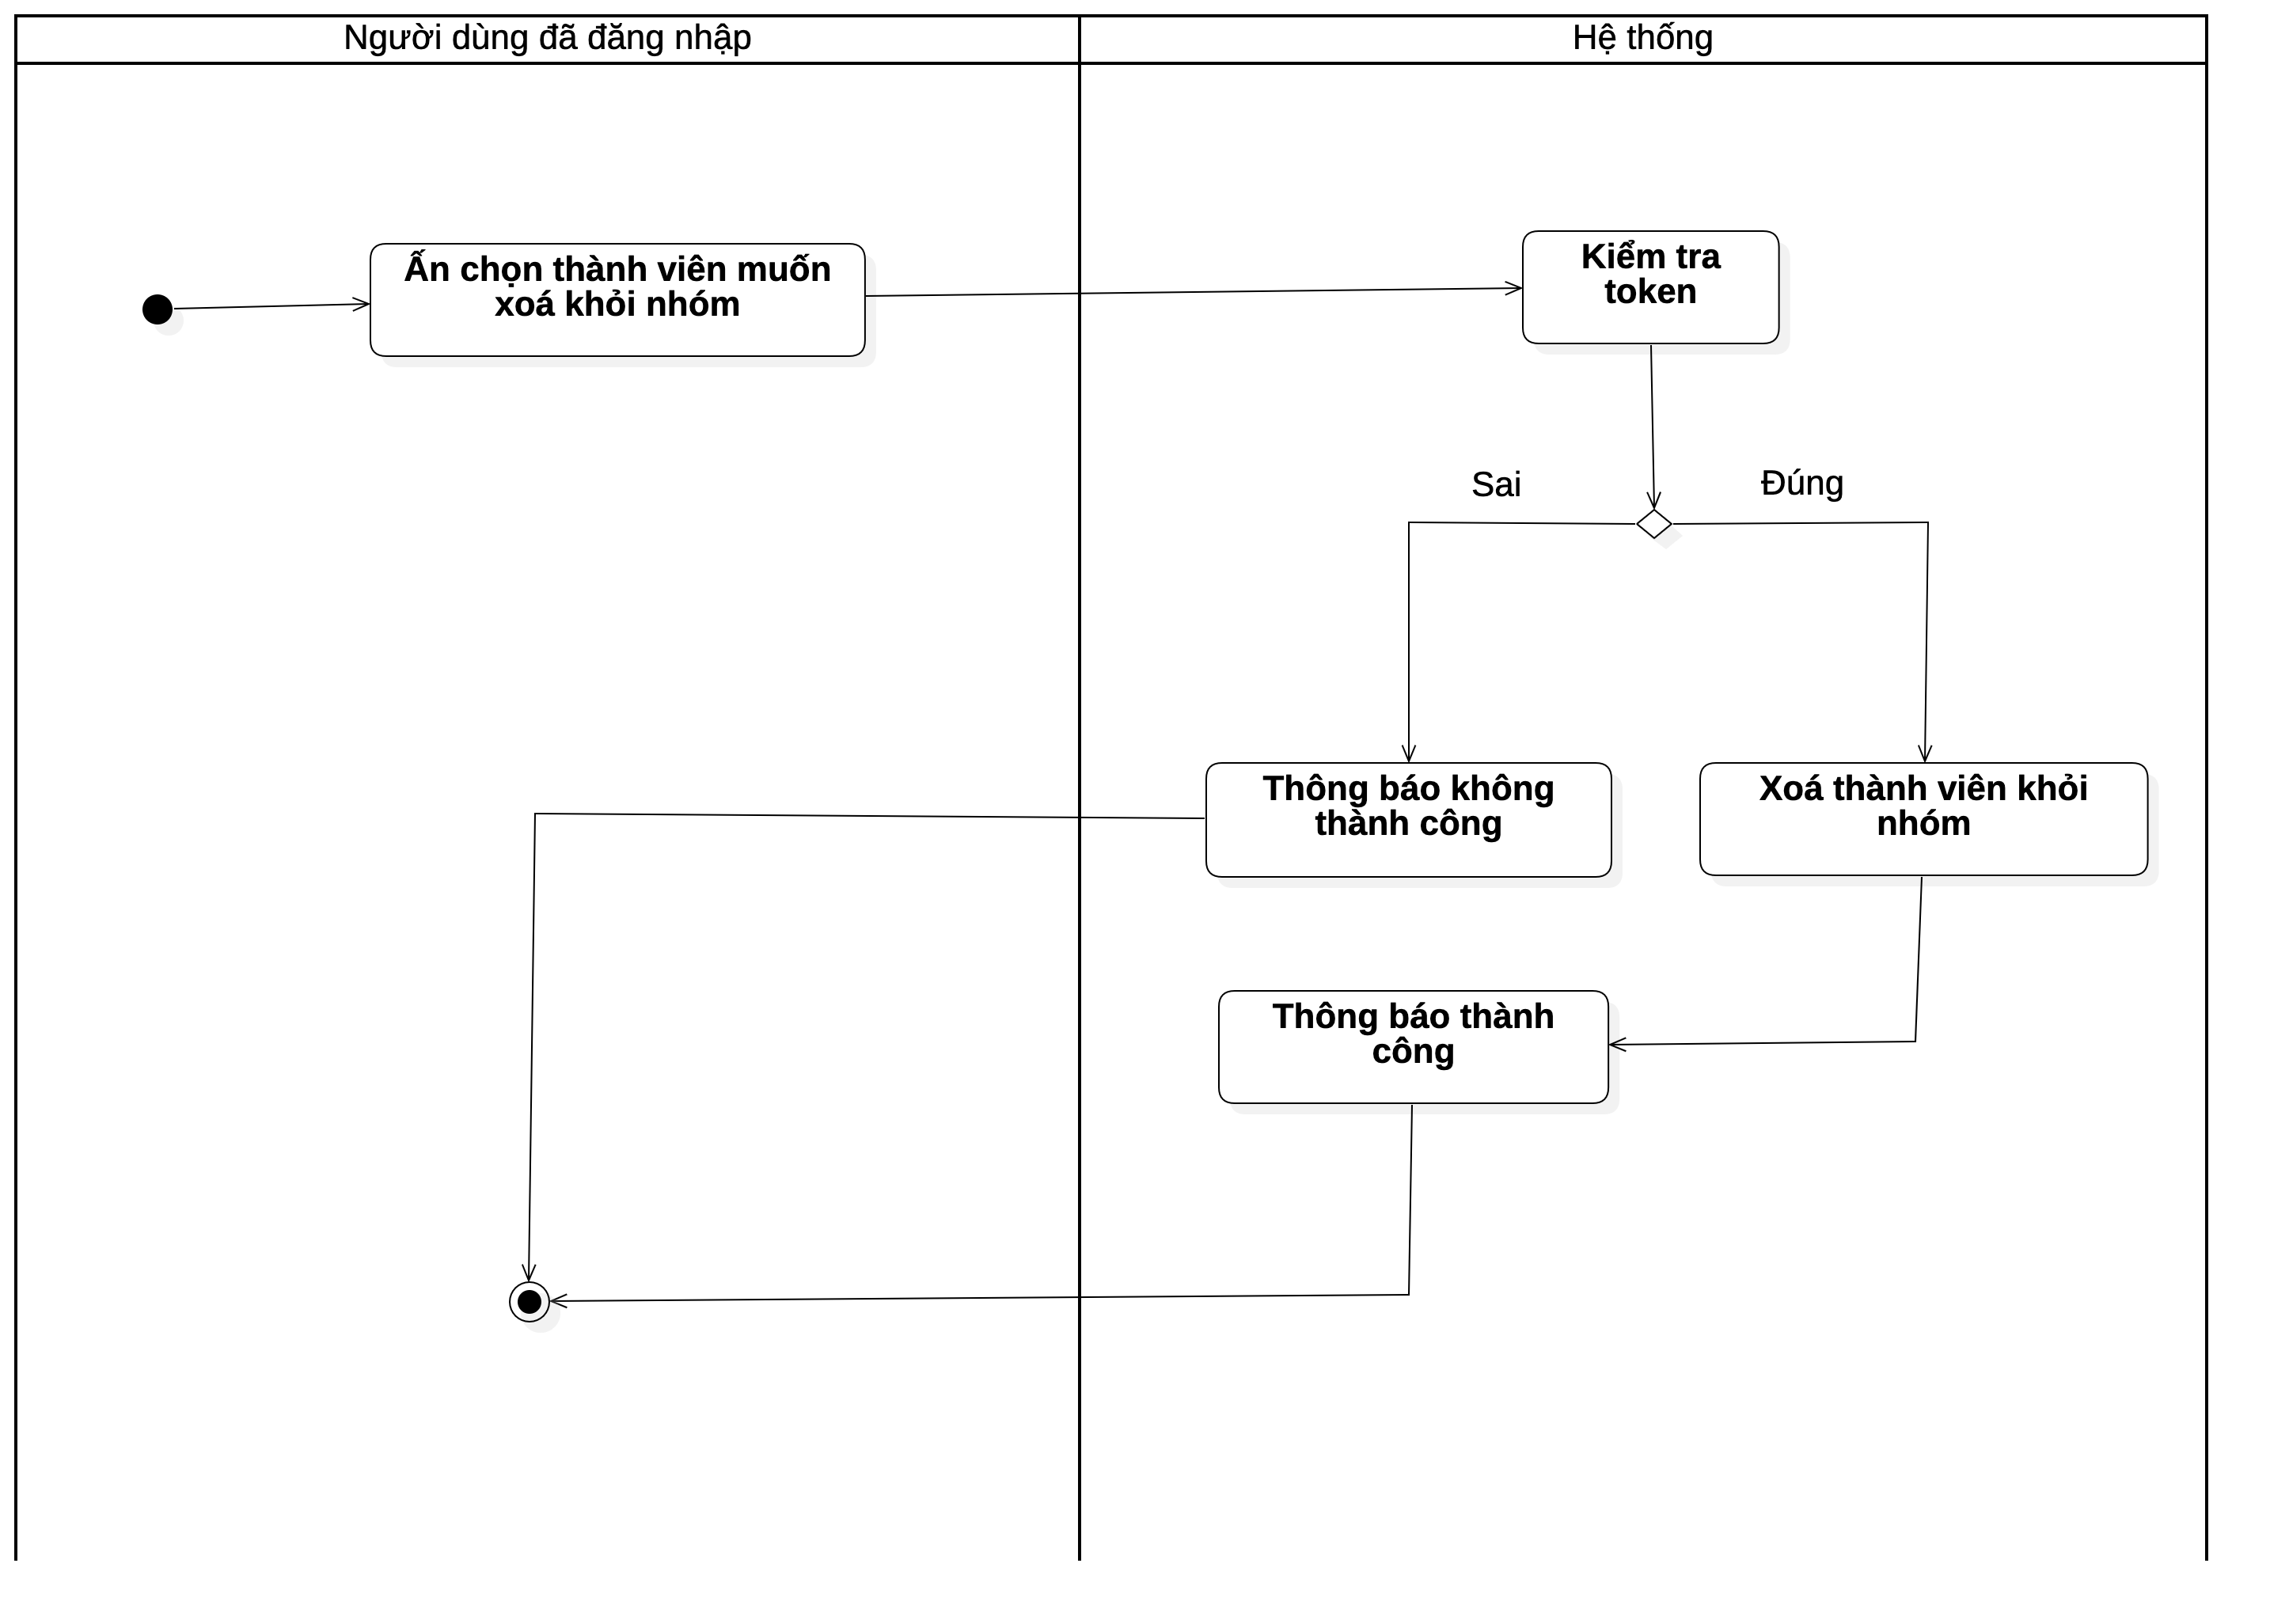
\includegraphics[width=0.9\linewidth]{Hinhve/Activity/Activity_Xoa_Thanh_Vien_Khoi_Nhom_Chat.png}
    \caption{Sơ đồ hoạt động quy trình nghiệp vụ Xoá thành viên khỏi nhóm chat}
    \label{fig:dang_nhap}
\end{figure}
\hfill

\subsection{Nghiệp vụ Gửi tin nhắn ảnh và video}
\begin{figure}[H]
   \centering
    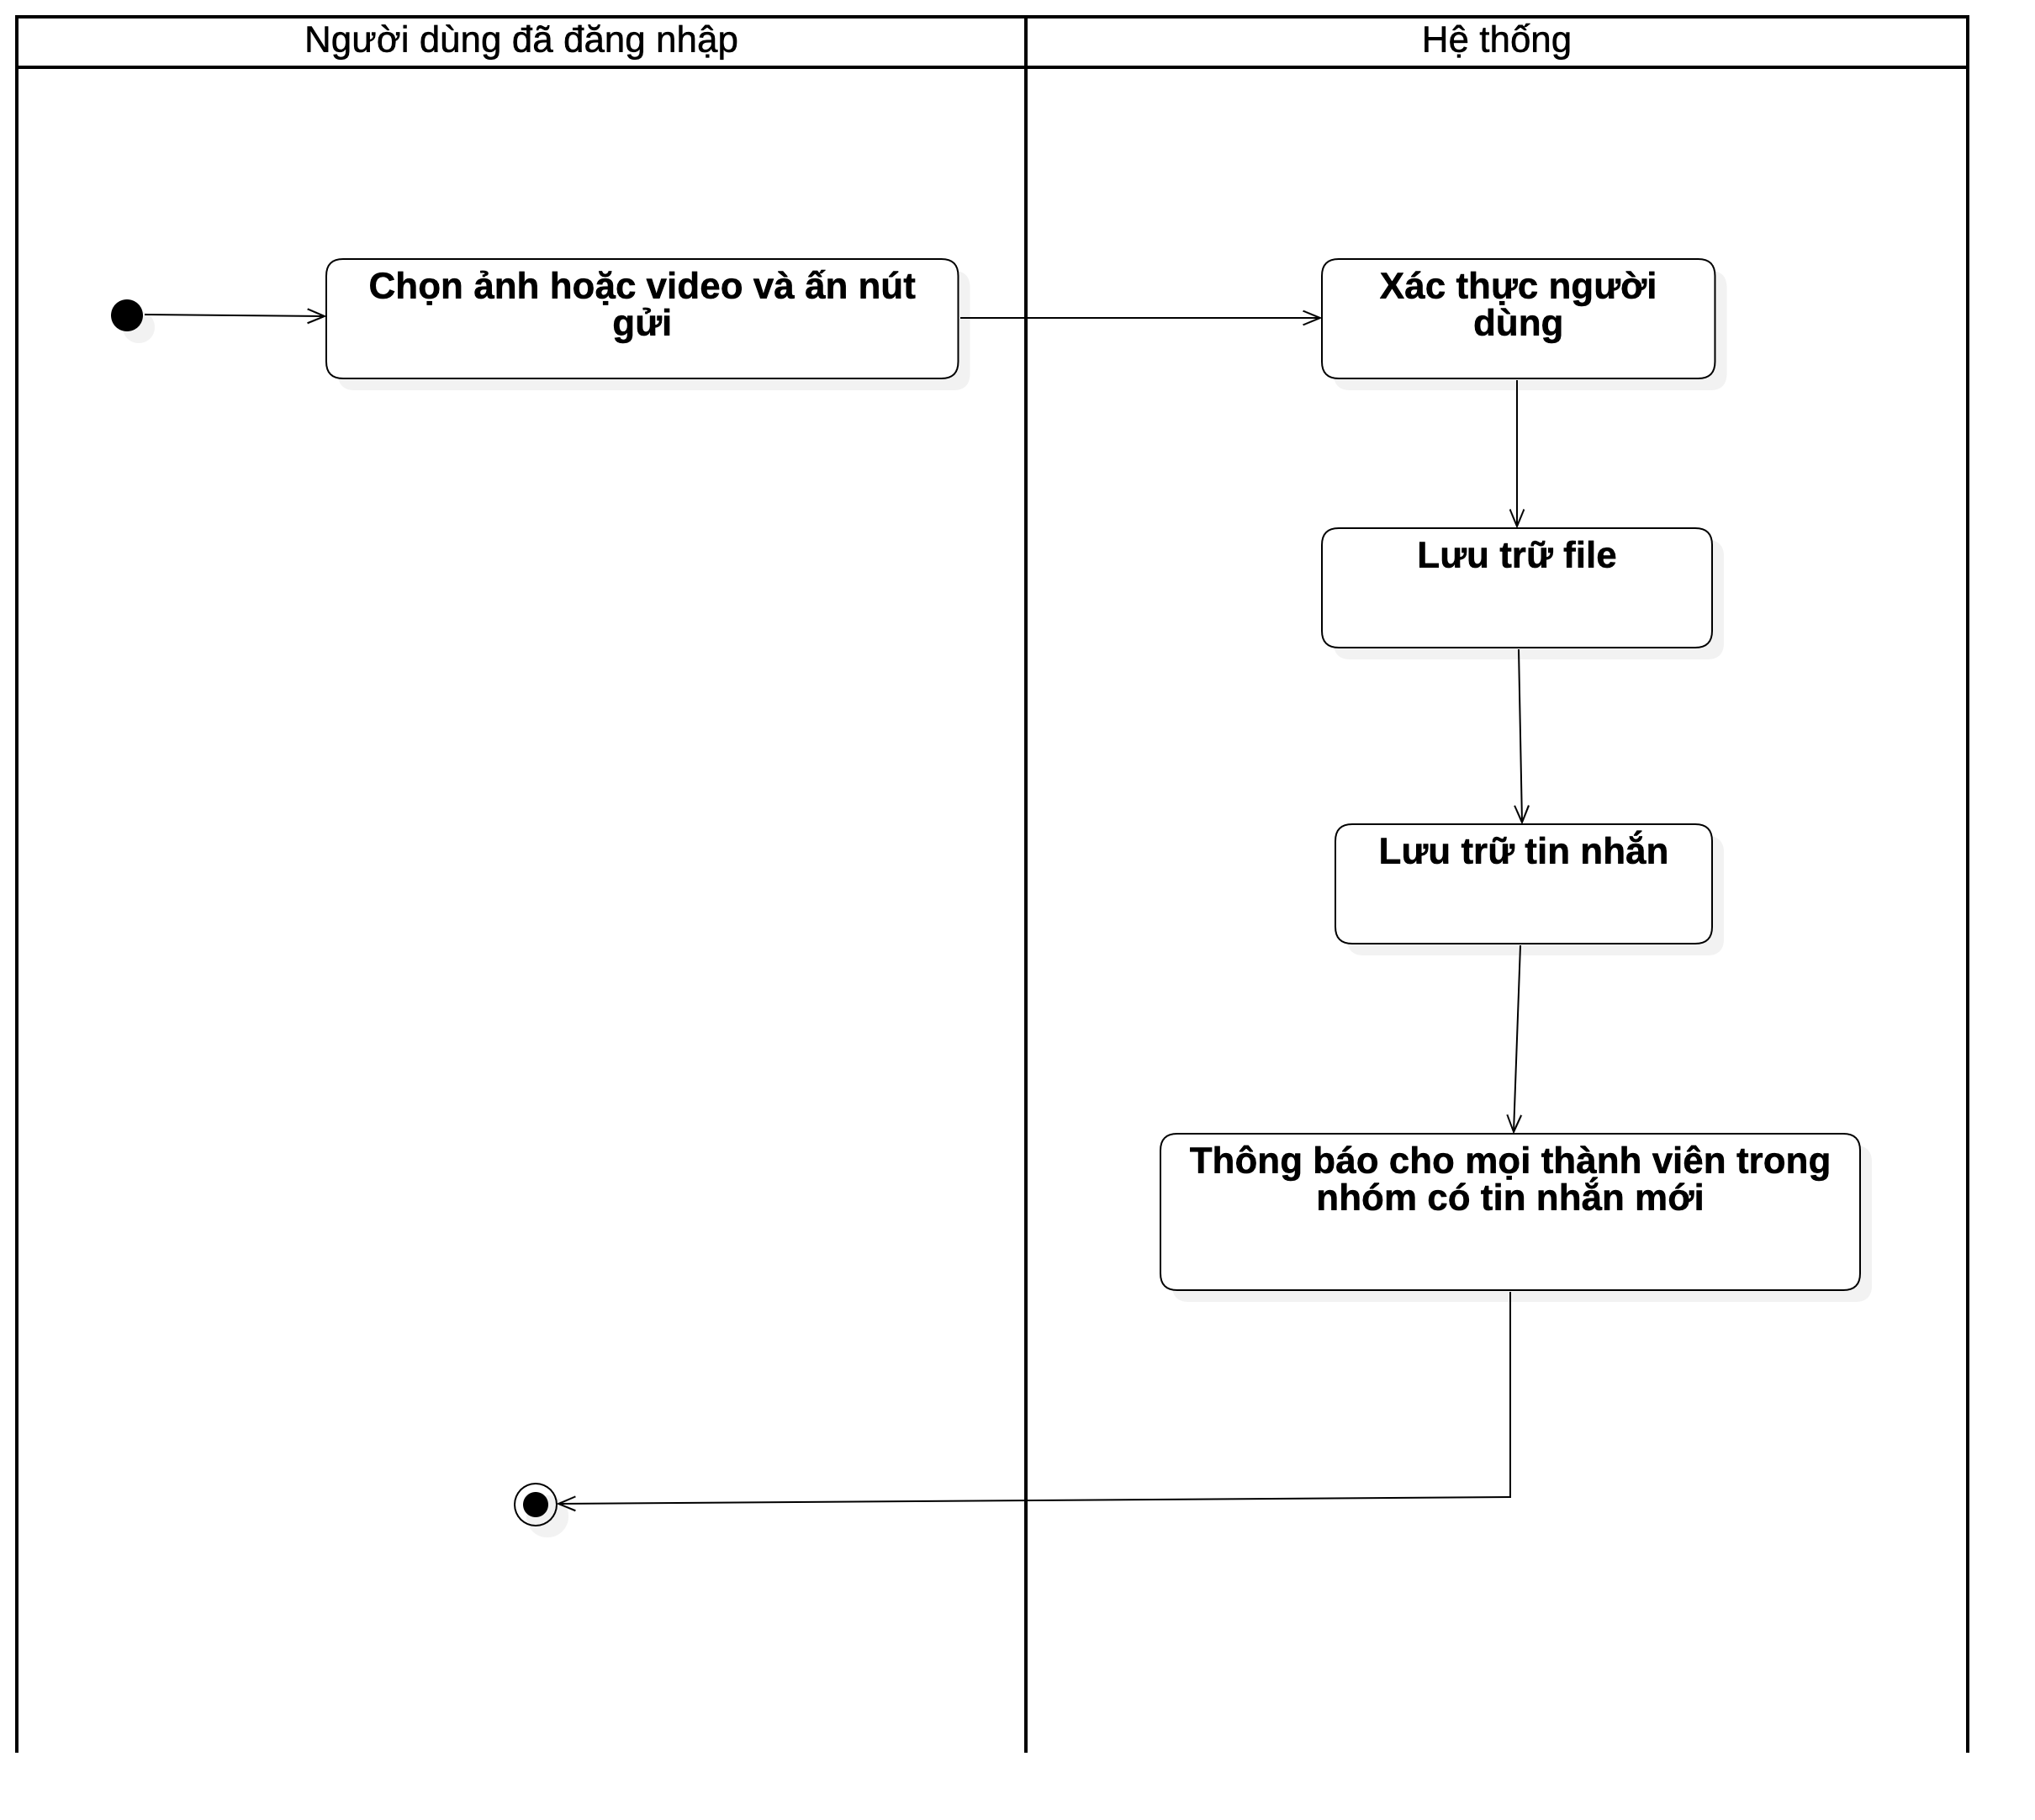
\includegraphics[width=1\linewidth]{Hinhve/Activity/Activity_Gui_Tin_Nhan_Anh_Va_Video.png}
    \caption{Sơ đồ hoạt động quy trình nghiệp vụ Gửi tin nhắn ảnh và video}
    \label{fig:dang_nhap}
\end{figure}
\hfill

\subsection{Nghiệp vụ Gửi tin nhắn văn bản}
\begin{figure}[H]
   \centering
    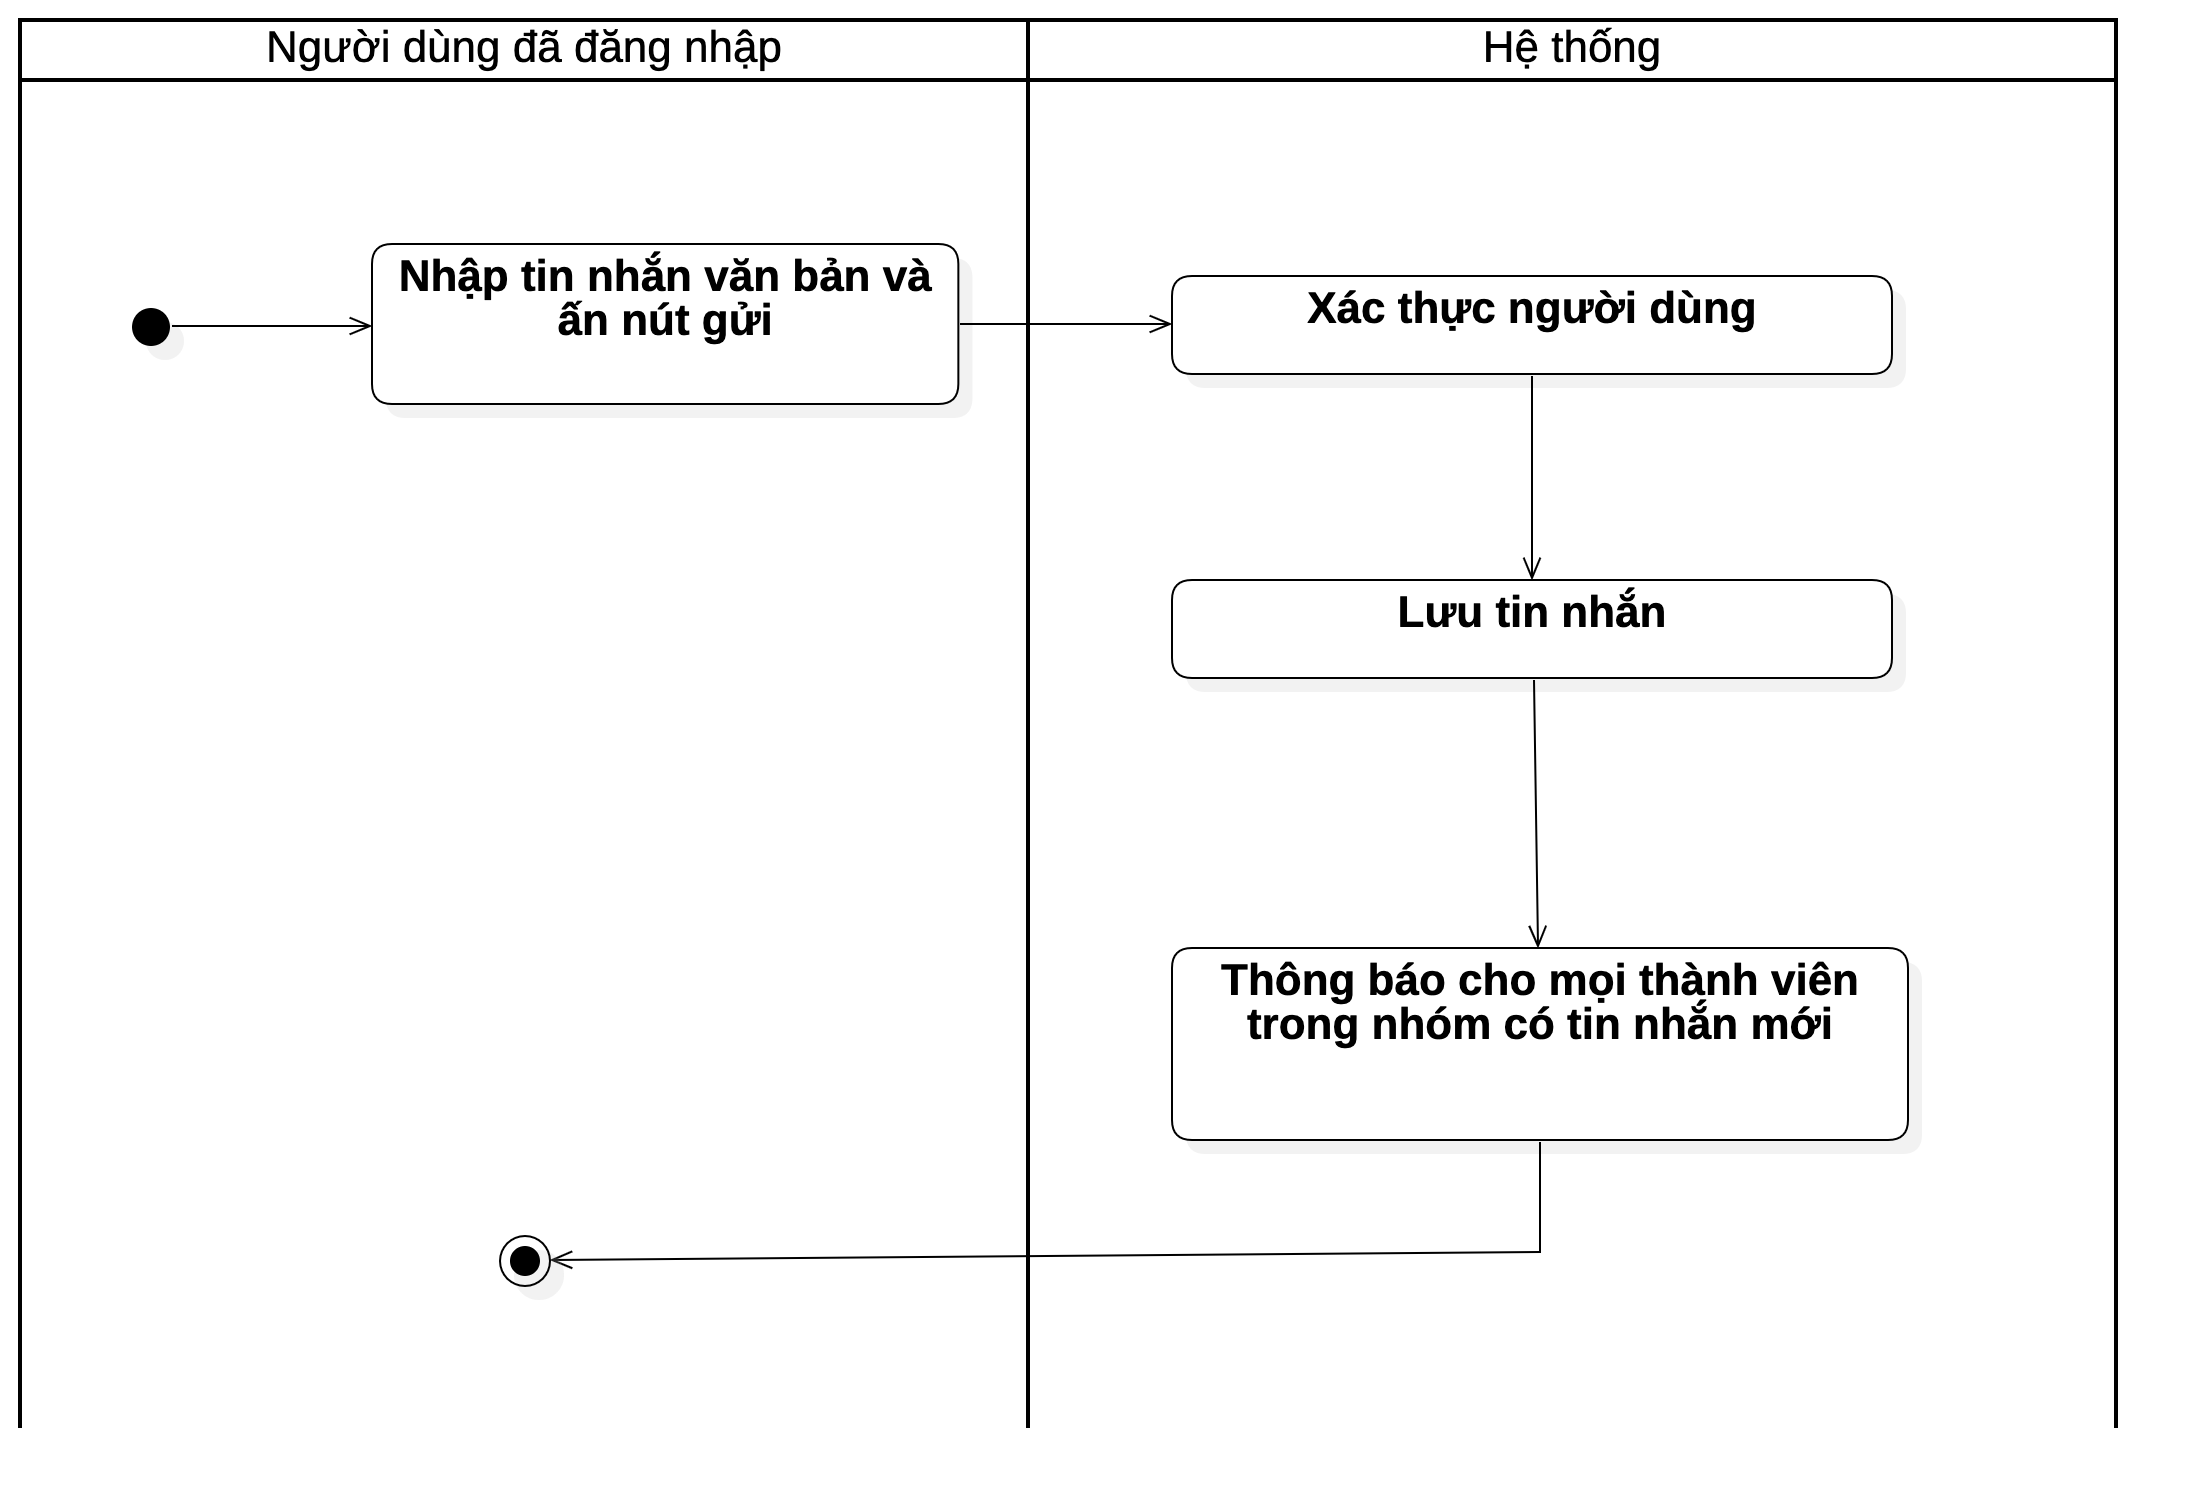
\includegraphics[width=1\linewidth]{Hinhve/Activity/Activity_Gui_Tin_Nhan_Van_Ban.png}
    \caption{Sơ đồ hoạt động quy trình nghiệp vụ Gửi tin nhắn văn bản}
    \label{fig:dang_nhap}
\end{figure}

\subsection{Nghiệp vụ Đăng xuất}
\begin{figure}[H]
   \centering
    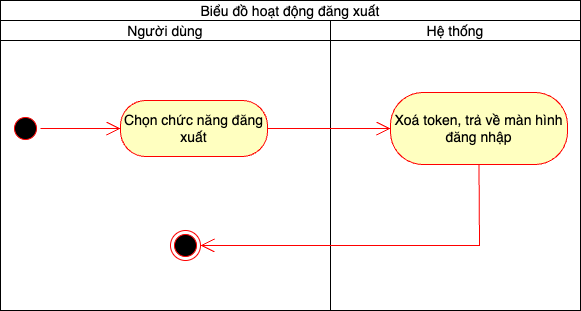
\includegraphics[width=1\linewidth]{Hinhve/Activity/dang_xuat.png}
    \caption{Sơ đồ hoạt động quy trình nghiệp vụ Đăng xuất}
    \label{fig:dang_xuat}
\end{figure} 
\newpage

\section{Đặc tả ca chức năng}
\label{section:2.4}
\subsection{Đặc cả use case Đăng ký}

\begin{longtable}{
|>{\raggedright\arraybackslash}m{0.15\linewidth}
|>{\raggedright\arraybackslash}m{0.15\linewidth}
|>{\raggedright\arraybackslash}m{0.2\linewidth}
|>{\raggedright\arraybackslash}m{0.4\linewidth}|}
    \hline
    \textbf{Mã usecase} & UC03 & \textbf{Tên Use case} & {Đăng ký} \\ \hline
    \textbf{Mô tả} & \multicolumn{3}{l|}{Cho phép người dùng đăng ký tài khoản trên hệ thống}\\ \hline
    \textbf{Tác nhân} & \multicolumn{3}{l|}{Người dùng}\\ \hline
    \textbf{Tiền điều kiện} & \multicolumn{3}{l|}{Không} \\ \hline
    \textbf{Sự kiện kích hoạt} & \multicolumn{3}{l|}{Người dùng click vào button “Đăng ký”}\\ \hline
    \textbf{Luồng sự kiện chính} & \multicolumn{3}{l|}{
    \begin{subtable}{0.8\linewidth}
        \centering
        \begin{tabular}{|>{\raggedright\arraybackslash}m{0.06\linewidth}|>{\raggedright\arraybackslash}m{0.24\linewidth}|>{\raggedright\arraybackslash}m{0.6\linewidth}|}
        \textbf{STT} & \textbf{Thực hiện} & \textbf{Hành động} \\
        \hline
        1 & Người dùng & Điền thông tin đăng ký \\ \hline
        2 & Người dùng & Gửi thông tin đăng ký \\ \hline
        3 & Hệ thống & Kiểm tra dữ liệu đầu vào \\ \hline
        4 & Hệ thống & Kiểm tra tên tài khoản xem đã tồn tại hay chưa \\ \hline
        5 & Hệ thống & Lưu tài khoản người dùng \\ \hline
        6 & Hệ thống & Hiển thị màn hình đăng nhập \\ \hline 
       \end{tabular}
    \end{subtable}
    \hfill
    }\\ \hline
     \textbf{Luồng sự kiện thay thế} & \multicolumn{3}{l|}{
    \begin{subtable}{0.8\linewidth}
        \centering
        \begin{tabular}{|>{\raggedright\arraybackslash}m{0.06\linewidth}|>{\raggedright\arraybackslash}m{0.24\linewidth}|>{\raggedright\arraybackslash}m{0.6\linewidth}|}
        \textbf{STT} & \textbf{Thực hiện} & \textbf{Hành động} \\
        \hline
        3a & Hệ thống & Thông báo lỗi: Yêu cầu người dùng kiểm tra lại thông tin tài khoản, mật khẩu và mật khẩu xác nhận đã nhập \\ \hline
        4a & Hệ thống & Thông báo lỗi: Đã có người dùng đăng ký tên tài khoản này \\ \hline
       \end{tabular}
    \end{subtable}
    \hfill
    } \\ \hline
     \textbf{Hậu điều kiện} & \multicolumn{3}{l|}{Hiển thị màn hình đăng nhập}\\ \hline
    \caption{Đặc tả usecase Đăng Ký}
    \label{table:usecaseDangNhap}
\end{longtable}

% \begin{figure}[H]
%    \centering
%     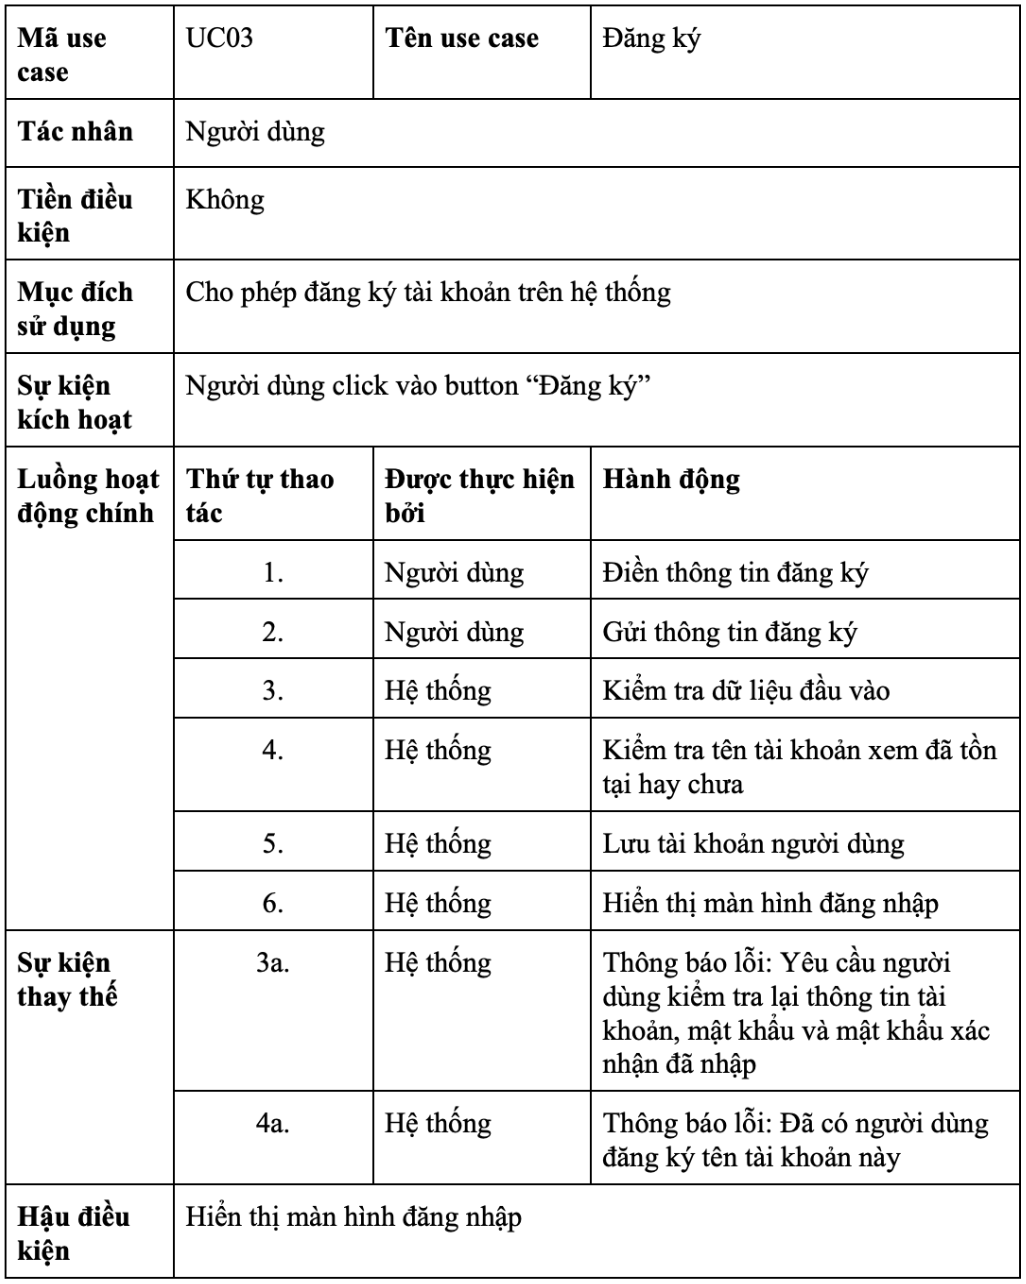
\includegraphics[width=1\linewidth]{Hinhve/UseCase/Specification/Dang_Ky.png}
%     \caption{Bảng đặc cả use case Đăng ký}
%     \label{fig:dang_xuat}
% \end{figure} 

\newpage
Danh sách các trường dữ liệu đầu vào form đăng ký:
\begin{longtable}[c]{
|>{\raggedright\arraybackslash}m{0.05\linewidth}
|>{\raggedright\arraybackslash}m{0.1\linewidth}
|>{\raggedright\arraybackslash}m{0.2\linewidth}
|>{\raggedright\arraybackslash}m{0.1\linewidth}
|>{\raggedright\arraybackslash}m{0.2\linewidth}
|>{\raggedright\arraybackslash}m{0.25\linewidth}|}
\hline
\textbf{Thứ tự} & \textbf{Trường dữ liệu} & \textbf{Mô tả} & \textbf{Bắt buộc} & \textbf{Yêu cầu hợp lệ} & \textbf{Ví dụ} \hline
\endfirsthead
1 & name & Tên của người dùng & Có & & Vũ Quý Đạt \\ \hline
2 & username & Tên năng nhập của người dùng & Có & Không có ký tự khoảng trắng & VuQuyDatk62 \\ \hline
3 & password & Mật khẩu & Có & Không có ký tự khoảng trắng & DatVQ.176082@ sis.hust.edu.vn \\ \hline
4 & confirm password & Mật khẩu xác nhận & Có & Không có ký tự khoảng trắng và phải trùng với Mật khẩu & DatVQ.176082@ sis.hust.edu.vn \\ \hline
5 & gender & giới tính của người dùng & Không & Hệ thống sẽ đưa 3 lựa chọn để người dùng chọn & Nam \\ \hline
6 & bio & Thông tin giới thiệu bản thân của người dùng & Không & & Tôi sinh năm 1999 đang làm việc tại công ty phát triển game trên iOS \\ \hline
7 & birth & Ngày tháng năm sinh của người dùng & Không & Định dạng ngày/tháng/năm & 02/09/1999 \\ \hline
8 & phone & Số điện thoại của người dùng & Không & Chỉ nhập số và không có ký tự khoảng trắng & 0899081299 \\ \hline
9 & email & Email của người dùng & Không & & datvq.176082@ sis.hust.edu.vn \\ \hline
10 & country & Quốc gia của người dùng & Không & & VN, Viet Nam \\ \hline
\caption{Bảng dữ liệu đầu vào usecase Đăng ký}
\label{tab:use_case_tổng_quan}
\end{longtable}
% \begin{figure}[H]
%    \centering
%     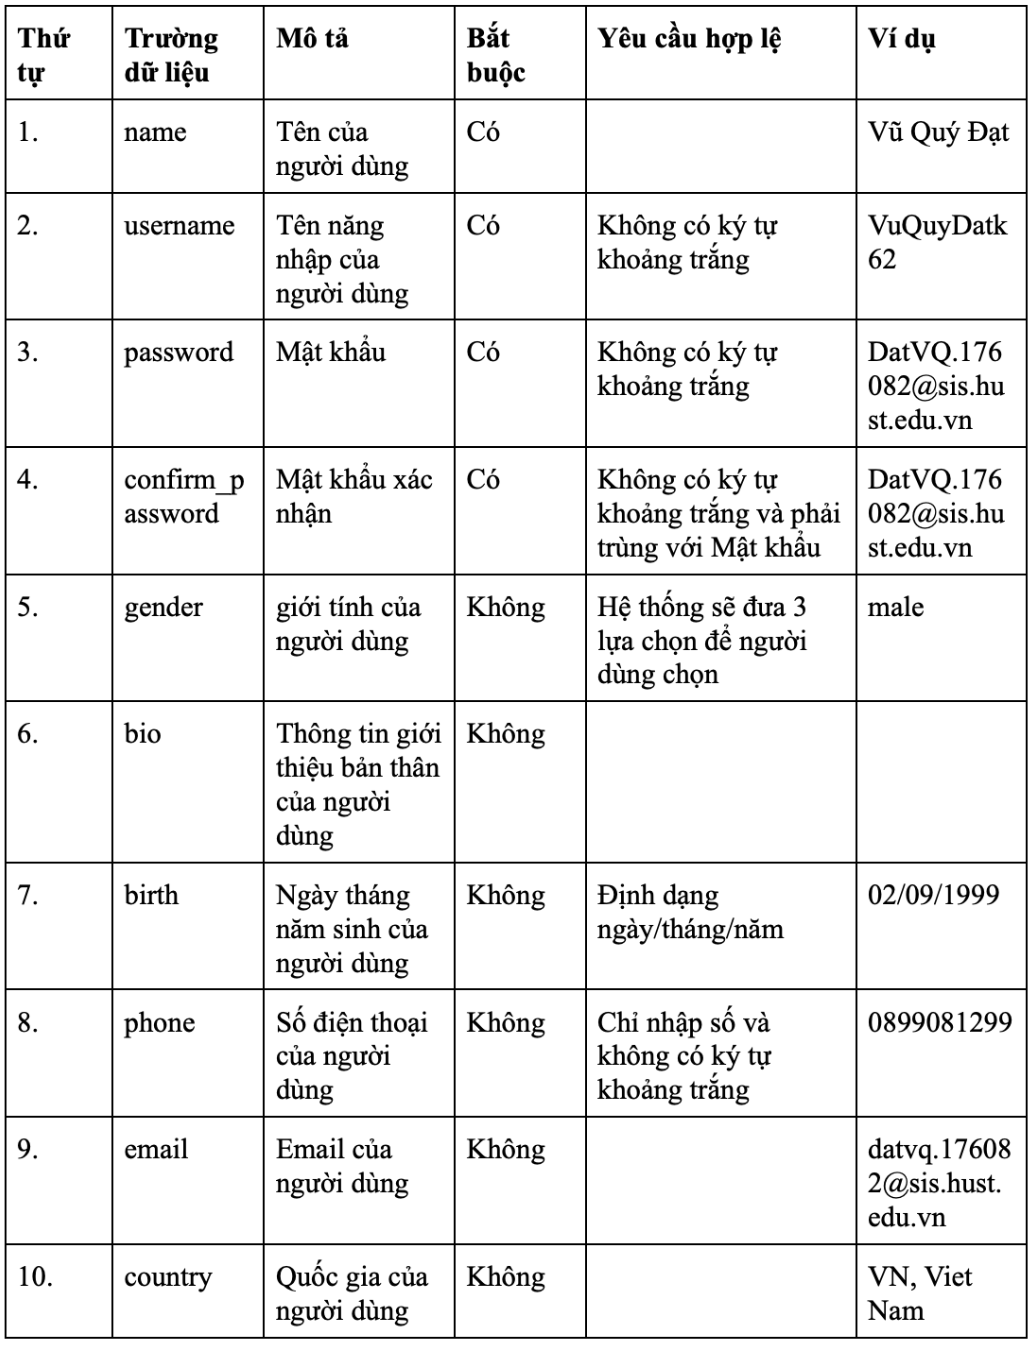
\includegraphics[width=1\linewidth]{Hinhve/UseCase/Specification/Dang_Ky_Data_Field.png}
%     \caption{Bảng dữ liệu đầu vào use case Đăng ký}
%     \label{fig:dang_xuat}
% \end{figure} 
\newpage

\subsection{Đặc cả use case Đăng nhập}
\begin{longtable}{
|>{\raggedright\arraybackslash}m{0.15\linewidth}
|>{\raggedright\arraybackslash}m{0.15\linewidth}
|>{\raggedright\arraybackslash}m{0.2\linewidth}
|>{\raggedright\arraybackslash}m{0.4\linewidth}|}
    \hline
    \textbf{Mã usecase} & UC01 & \textbf{Tên Use case} & {Đăng nhập} \\ \hline
    \textbf{Mô tả} & \multicolumn{3}{l|}{Cho phép đăng nhập vào hệ thống và sử dụng các chức năng}\\ \hline
    \textbf{Tác nhân} & \multicolumn{3}{l|}{Người dùng}\\ \hline
    \textbf{Tiền điều kiện} & \multicolumn{3}{l|}{Người dùng đã có tài khoản được đăng ký thành công} \\ \hline
    \textbf{Sự kiện kích hoạt} & \multicolumn{3}{l|}{Người dùng click vào button “Đăng nhập”}\\ \hline
    \textbf{Luồng sự kiện chính} & \multicolumn{3}{l|}{
    \begin{subtable}{0.8\linewidth}
        \centering
        \begin{tabular}{|>{\raggedright\arraybackslash}m{0.06\linewidth}|>{\raggedright\arraybackslash}m{0.24\linewidth}|>{\raggedright\arraybackslash}m{0.6\linewidth}|}
        \textbf{STT} & \textbf{Thực hiện} & \textbf{Hành động} \\
        \hline
        1 & Hệ thống & Kiểm tra token đã tồn tại hay chưa \\ \hline
        2 & Người dùng & Điền thông tin đăng nhập \\ \hline
        3 & Người dùng & Gửi yêu cầu đăng nhập \\ \hline
        4 & Hệ thống & Hiển thị màn hình chờ và kiểm tra dữ liệu đầu vào \\ \hline
        5 & Hệ thống & Kiểm tra xem tài khoản đã tồn tại hay chưa \\ \hline
        6 & Hệ thống & Sinh token và lưu token \\ \hline 
        7 & Hệ thống & Ẩn màn hình chờ và hiển thị màn hình trang chủ (màn hình danh sách người dùng) \\ \hline 
       \end{tabular}
    \end{subtable}
    \hfill
    }\\ \hline
     \textbf{Luồng sự kiện thay thế} & \multicolumn{3}{l|}{
    \begin{subtable}{0.8\linewidth}
        \centering
        \begin{tabular}{|>{\raggedright\arraybackslash}m{0.06\linewidth}|>{\raggedright\arraybackslash}m{0.24\linewidth}|>{\raggedright\arraybackslash}m{0.6\linewidth}|}
        \textbf{STT} & \textbf{Thực hiện} & \textbf{Hành động} \\
        \hline
        1a & Hệ thống & Hiển thị màn hình trang chủ (màn hình danh sách người dùng) \\ \hline
        4a & Hệ thống & Thông báo lỗi: Yêu cầu người dùng kiểm tra lại thông tin tài khoản và mật khẩu đã nhập. Ẩn màn hình chờ và hiển thị màn hình đăng nhập \\ \hline
        5a & Hệ thống & Thông báo lỗi: Đăng nhập không thành công. Ẩn màn hình chờ và hiển thị màn hình đăng nhập \\ \hline
       \end{tabular}
    \end{subtable}
    \hfill
    } \\ \hline
     \textbf{Hậu điều kiện} & \multicolumn{3}{l|}{Hiển thị màn hình trang chủ}\\ \hline
    \caption{Đặc tả usecase Đăng Nhập}
    \label{table:usecaseDangNhap}
\end{longtable}
% \begin{figure}[H]
%    \centering
%     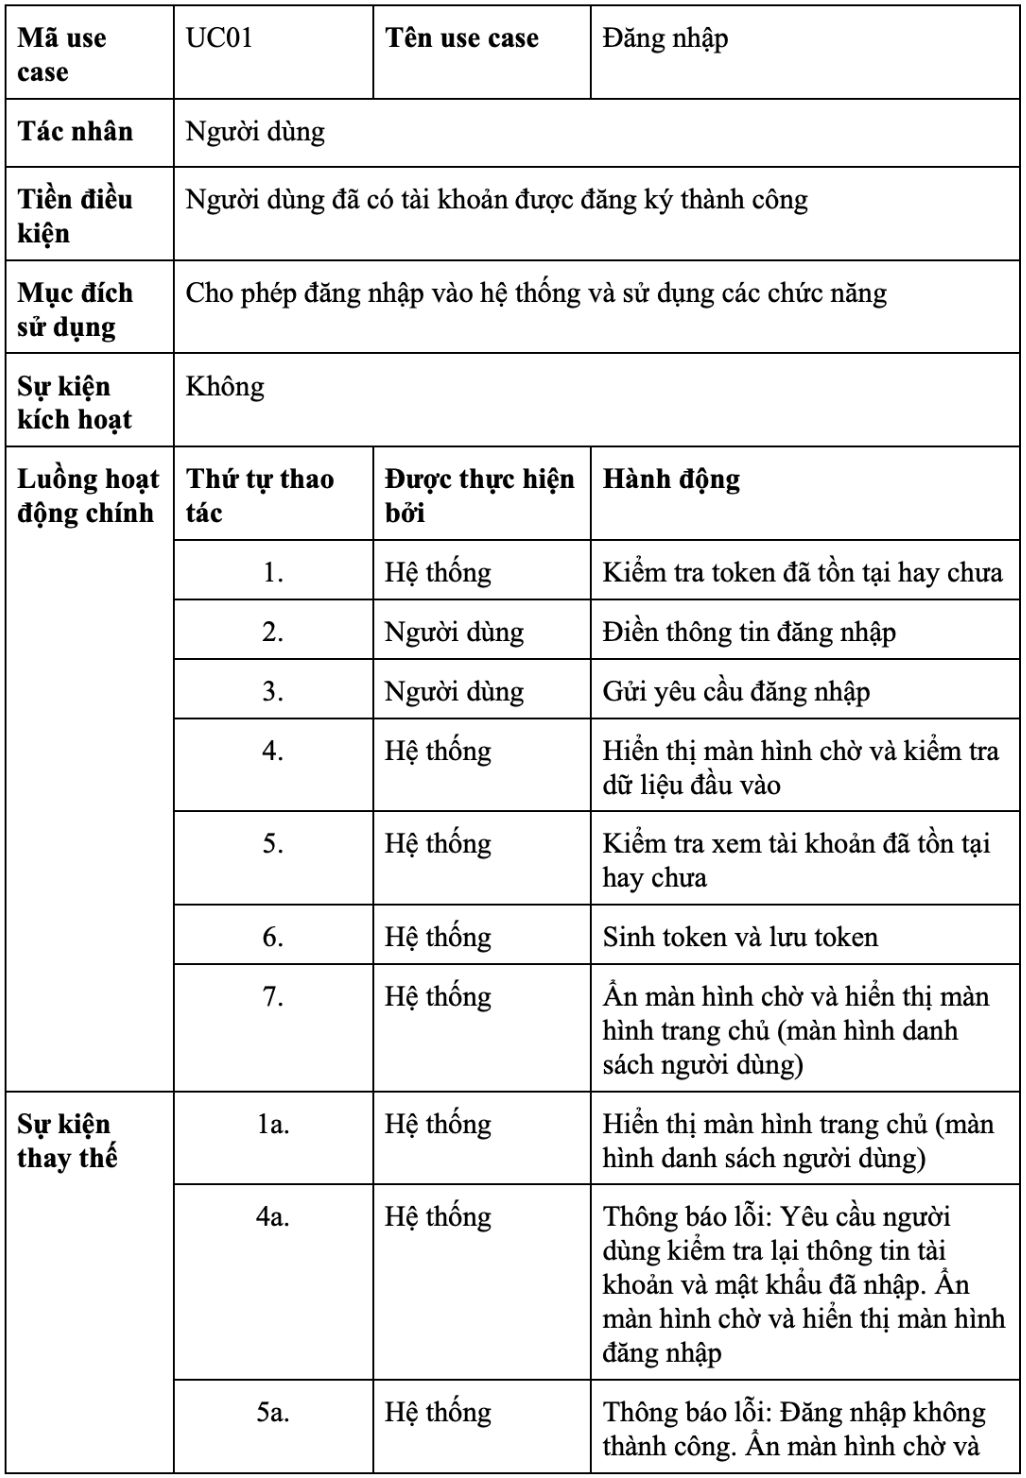
\includegraphics[width=1\linewidth]{Hinhve/UseCase/Specification/Dang_Nhap.png}
%     \caption{Bảng đặc cả use case Đăng nhập}
%     \label{fig:dang_xuat}
% \end{figure} 

\newpage
Danh sách các trường dữ liệu đầu vào form đăng nhập:
\begin{longtable}[c]{
|>{\raggedright\arraybackslash}m{0.05\linewidth}
|>{\raggedright\arraybackslash}m{0.1\linewidth}
|>{\raggedright\arraybackslash}m{0.2\linewidth}
|>{\raggedright\arraybackslash}m{0.1\linewidth}
|>{\raggedright\arraybackslash}m{0.2\linewidth}
|>{\raggedright\arraybackslash}m{0.25\linewidth}|}
\hline
\textbf{Thứ tự} & \textbf{Trường dữ liệu} & \textbf{Mô tả} & \textbf{Bắt buộc} & \textbf{Yêu cầu hợp lệ} & \textbf{Ví dụ} \hline
\endfirsthead
1 & username & Tên năng nhập của người dùng & Có & Không có ký tự khoảng trắng & VuQuyDatk62 \\ \hline
2 & password & Mật khẩu & Có & Không có ký tự khoảng trắng & DatVQ.176082 \\ \hline
\caption{Bảng dữ liệu đầu vào usecase Đăng nhập}
\label{tab:use_case_tổng_quan}
\end{longtable}
% \begin{figure}[H]
%    \centering
%     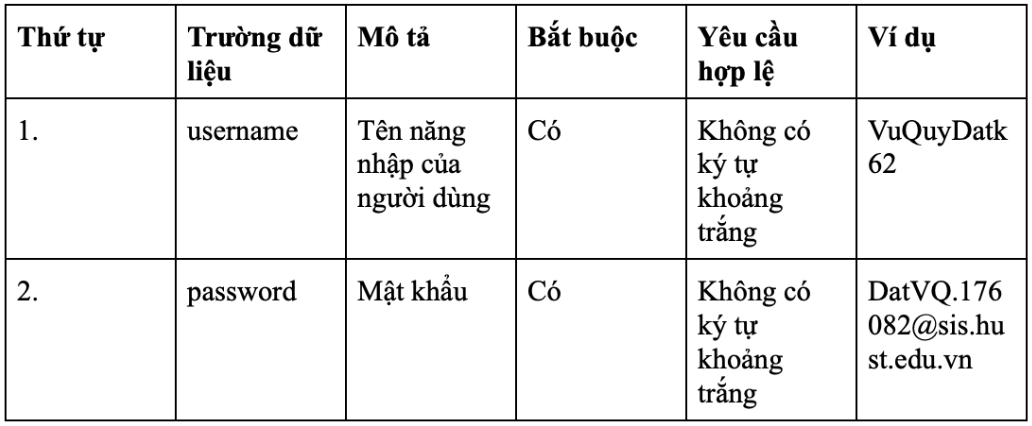
\includegraphics[width=1\linewidth]{Hinhve/UseCase/Specification/Dang_Nhap_Data_Field.png}
%     \caption{Bảng dữ liệu đầu vào use case Đăng nhập}
%     \label{fig:dang_xuat}
% \end{figure} 
\hfill


\subsection{Đặc cả use case Đăng xuất}
\begin{longtable}{
|>{\raggedright\arraybackslash}m{0.15\linewidth}
|>{\raggedright\arraybackslash}m{0.15\linewidth}
|>{\raggedright\arraybackslash}m{0.2\linewidth}
|>{\raggedright\arraybackslash}m{0.4\linewidth}|}
    \hline
    \textbf{Mã usecase} & UC02 & \textbf{Tên Use case} & {Đăng xuất} \\ \hline
    \textbf{Mô tả} & \multicolumn{3}{l|}{Cho phép người dùng đăng xuất khỏi hệ thống}\\ \hline
    \textbf{Tác nhân} & \multicolumn{3}{l|}{Người dùng}\\ \hline
    \textbf{Tiền điều kiện} & \multicolumn{3}{l|}{Người dùng đã đăng nhập vào hệ thống} \\ \hline
    \textbf{Sự kiện kích hoạt} & \multicolumn{3}{l|}{Người dùng click vào button “Đăng xuất”}\\ \hline
    \textbf{Luồng sự kiện chính} & \multicolumn{3}{l|}{
    \begin{subtable}{0.8\linewidth}
        \centering
        \begin{tabular}{|>{\raggedright\arraybackslash}m{0.06\linewidth}|>{\raggedright\arraybackslash}m{0.24\linewidth}|>{\raggedright\arraybackslash}m{0.6\linewidth}|}
        \textbf{STT} & \textbf{Thực hiện} & \textbf{Hành động} \\
        \hline
        1 & Người dùng & Click vào button “Đăng xuất” \\ \hline
        2 & Hệ thống & Xoá token, hiển thị màn hình đăng nhập \\ \hline
       \end{tabular}
    \end{subtable}
    \hfill
    }\\ \hline
     \textbf{Luồng sự kiện thay thế} & \multicolumn{3}{l|}{
    \begin{subtable}{0.8\linewidth}
        % \centering
        Không
    \end{subtable}
    \hfill
    } \\ \hline
     \textbf{Hậu điều kiện} & \multicolumn{3}{l|}{Đăng xuất người dùng khỏi hệ thống, hiển thị màn hình đăng nhập}\\ \hline
    \caption{Đặc tả usecase Đăng xuất}
    \label{table:usecaseDangNhap}
\end{longtable}
% \begin{figure}[H]
%    \centering
%     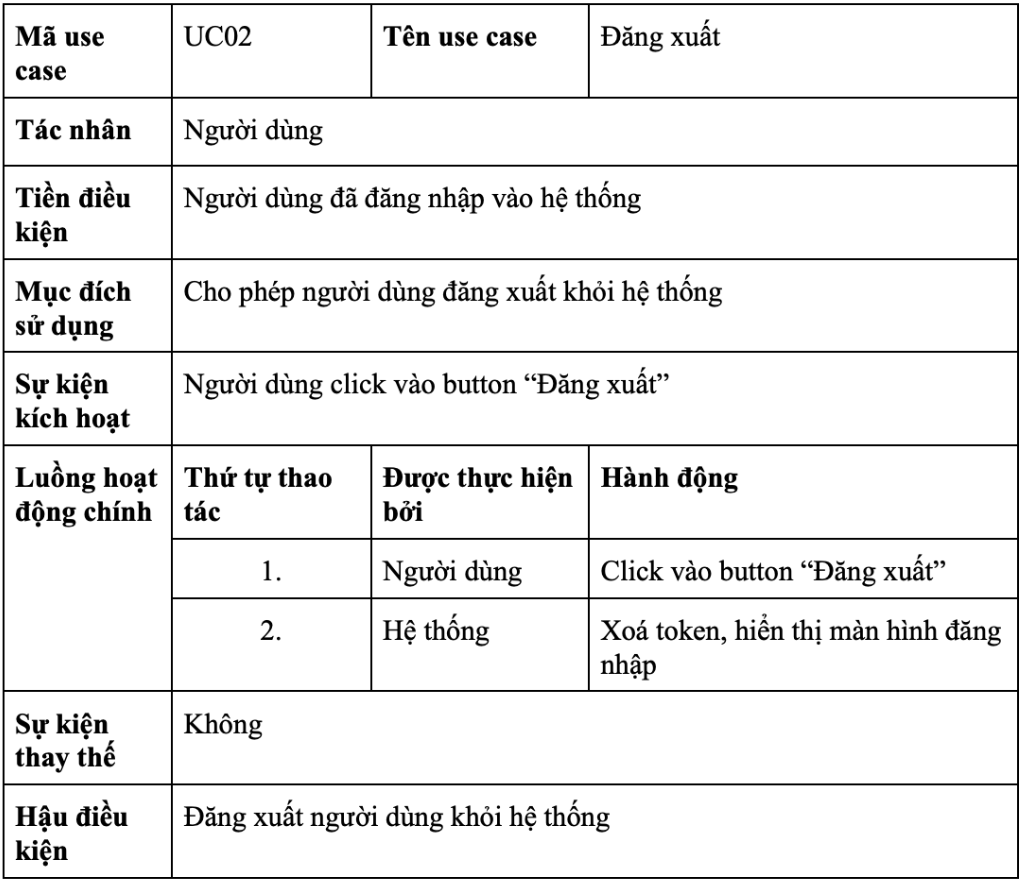
\includegraphics[width=1\linewidth]{Hinhve/UseCase/Specification/Dang_Xuat.png}
%     \caption{Bảng đặc cả use case Đăng xuất}
%     \label{fig:dang_xuat}
% \end{figure} 
\newpage

\subsection{Đặc cả use case Gửi tin nhắn}
\begin{longtable}{
|>{\raggedright\arraybackslash}m{0.15\linewidth}
|>{\raggedright\arraybackslash}m{0.15\linewidth}
|>{\raggedright\arraybackslash}m{0.2\linewidth}
|>{\raggedright\arraybackslash}m{0.4\linewidth}|}
    \hline
    \textbf{Mã usecase} & UC04 & \textbf{Tên Use case} & {Gửi tin nhắn} \\ \hline
    \textbf{Mô tả} & \multicolumn{3}{l|}{Gửi tin nhắn văn bản, tin nhắn ảnh, tin nhắn video}\\ \hline
    \textbf{Tác nhân} & \multicolumn{3}{l|}{Người dùng}\\ \hline
    \textbf{Tiền điều kiện} & \multicolumn{3}{l|}{Người dùng đã đăng nhập, tồn tại chat box với người muốn gửi tin nhắn} \\ \hline
    \textbf{Sự kiện kích hoạt} & \multicolumn{3}{l|}{Người dùng click vào button “Gửi”}\\ \hline
    \textbf{Luồng sự kiện chính} & \multicolumn{3}{l|}{
    \begin{subtable}{0.8\linewidth}
        \centering
        \begin{tabular}{|>{\raggedright\arraybackslash}m{0.06\linewidth}|>{\raggedright\arraybackslash}m{0.24\linewidth}|>{\raggedright\arraybackslash}m{0.6\linewidth}|}
        \textbf{STT} & \textbf{Thực hiện} & \textbf{Hành động} \\
        \hline
        1 & Người dùng & Nhập văn bản hoặc chọn ảnh, video \\ \hline
        2 & Người dùng & Click vào button “Gửi” \\ \hline
        3 & Hệ thống & Kiểm tra dữ liệu đầu vào \\ \hline
        4 & Hệ thống & Lưu tin nhắn \\ \hline
        5 & Hệ thống & Hiển thị tin nhắn mới trên màn hình nhắn tin \\ \hline
       \end{tabular}
    \end{subtable}
    \hfill
    }\\ \hline
     \textbf{Luồng sự kiện thay thế} & \multicolumn{3}{l|}{
    \begin{subtable}{0.8\linewidth}
        % \centering
        Không
    \end{subtable}
    \hfill
    } \\ \hline
     \textbf{Hậu điều kiện} & \multicolumn{3}{l|}{Đồng bộ dữ liệu tin nhắn và hiển thị}\\ \hline
    \caption{Đặc tả usecase Gửi tin nhắn}
    \label{table:usecaseDangNhap}
\end{longtable}
% \begin{figure}[H]
%    \centering
%     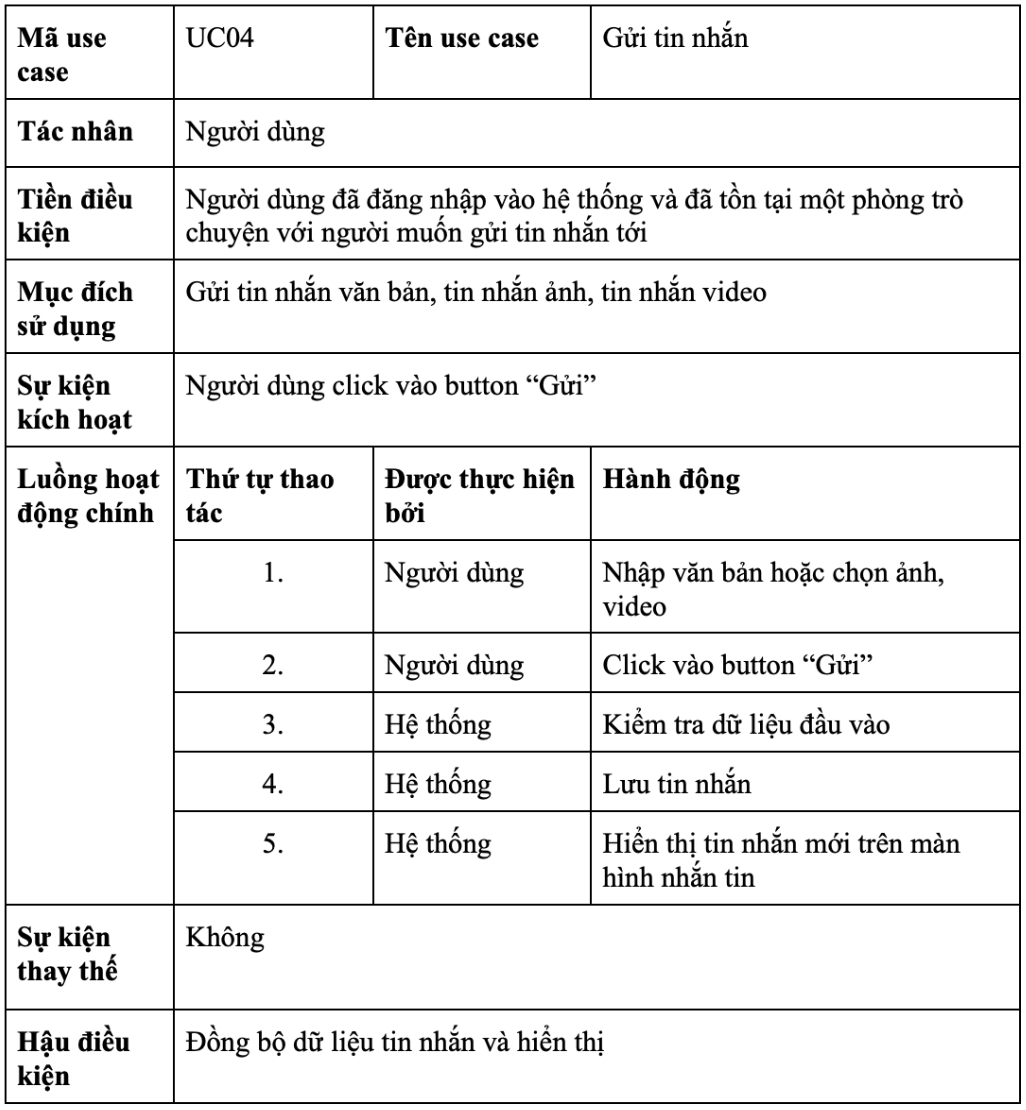
\includegraphics[width=1\linewidth]{Hinhve/UseCase/Specification/Gui_Tin_Nhan.png}
%     \caption{Bảng đặc cả use case Gửi tin nhắn}
%     \label{fig:dang_xuat}
% \end{figure} 

Danh sách các trường dữ liệu đầu vào form Gửi tin nhắn:
\begin{longtable}[c]{
|>{\raggedright\arraybackslash}m{0.05\linewidth}
|>{\raggedright\arraybackslash}m{0.1\linewidth}
|>{\raggedright\arraybackslash}m{0.2\linewidth}
|>{\raggedright\arraybackslash}m{0.1\linewidth}
|>{\raggedright\arraybackslash}m{0.2\linewidth}
|>{\raggedright\arraybackslash}m{0.25\linewidth}|}
\hline
\textbf{Thứ tự} & \textbf{Trường dữ liệu} & \textbf{Mô tả} & \textbf{Bắt buộc} & \textbf{Yêu cầu hợp lệ} & \textbf{Ví dụ} \hline
\endfirsthead
1 & content & Tin nhắn văn bản mà người dùng nhập vào & Có & & “Đây là nội dung của tin nhắn văn bản” \\ \hline
2 & data & Ảnh hoặc video mà người dùng đã chọn & Không & & \\ \hline
\caption{Bảng dữ liệu đầu vào usecase Gửi tin nhắn}
\label{tab:use_case_tổng_quan}
\end{longtable}
% \begin{figure}[H]
%    \centering
%     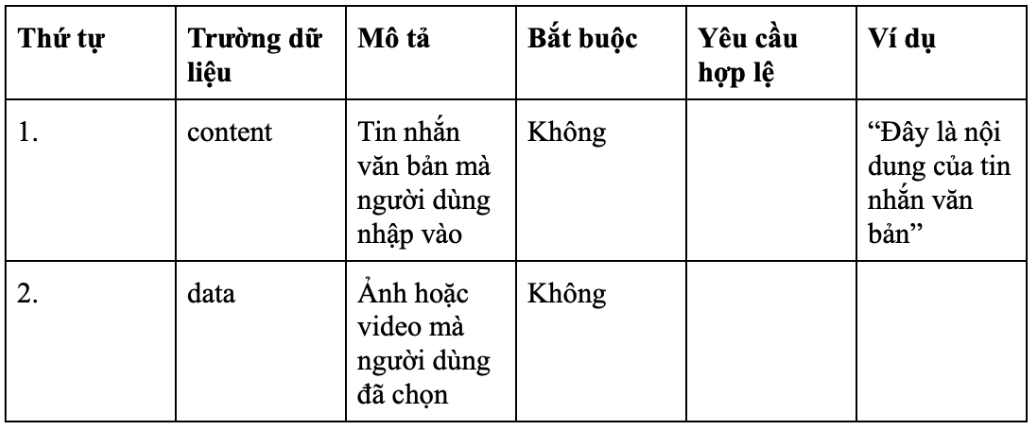
\includegraphics[width=1\linewidth]{Hinhve/UseCase/Specification/Gui_Tin_Nhan_Data_Field.png}
%     \caption{Bảng dữ liệu đầu vào use case Gửi tin nhắn}
%     \label{fig:dang_xuat}
% \end{figure} 

\newpage
\subsection{Đặc cả use case Thêm người dùng vào phòng chat}
\begin{longtable}{
|>{\raggedright\arraybackslash}m{0.15\linewidth}
|>{\raggedright\arraybackslash}m{0.15\linewidth}
|>{\raggedright\arraybackslash}m{0.2\linewidth}
|>{\raggedright\arraybackslash}m{0.4\linewidth}|}
    \hline
    \textbf{Mã usecase} & UC05 & \textbf{Tên Use case} & {Thêm người dùng vào phòng chat} \\ \hline
    \textbf{Mô tả} & \multicolumn{3}{l|}{Cho phép thêm người dùng khác vào phòng chat đang tồn tại}\\ \hline
    \textbf{Tác nhân} & \multicolumn{3}{l|}{Người dùng}\\ \hline
    \textbf{Tiền điều kiện} & \multicolumn{3}{l|}{Người dùng đã đăng nhập vào hệ thống} \\ \hline
    \textbf{Sự kiện kích hoạt} & \multicolumn{3}{l|}{Người dùng click vào button “Thêm”}\\ \hline
    \textbf{Luồng sự kiện chính} & \multicolumn{3}{l|}{
    \begin{subtable}{0.8\linewidth}
        \centering
        \begin{tabular}{|>{\raggedright\arraybackslash}m{0.06\linewidth}|>{\raggedright\arraybackslash}m{0.24\linewidth}|>{\raggedright\arraybackslash}m{0.6\linewidth}|}
        \textbf{STT} & \textbf{Thực hiện} & \textbf{Hành động} \\
        \hline
        1 & Người dùng & Chọn danh sách người dùng muốn thêm \\ \hline
        2 & Người dùng & Click vào button “Thêm” \\ \hline
        3 & Hệ thống & Thêm người dùng vào nhóm \\ \hline
       \end{tabular}
    \end{subtable}
    \hfill
    } \\ \hline
     \textbf{Luồng sự kiện thay thế} & \multicolumn{3}{l|}{
    \begin{subtable}{0.8\linewidth}
        Không
    \end{subtable}
    \hfill
    } \\ \hline
     \textbf{Hậu điều kiện} & \multicolumn{3}{l|}{Đồng bộ dữ liệu phòng chat và hiển thị}\\ \hline
    \caption{Đặc tả usecase Thêm người dùng vào phòng chat}
    \label{table:usecaseDangNhap}
\end{longtable}
% \begin{figure}[H]
%    \centering
%     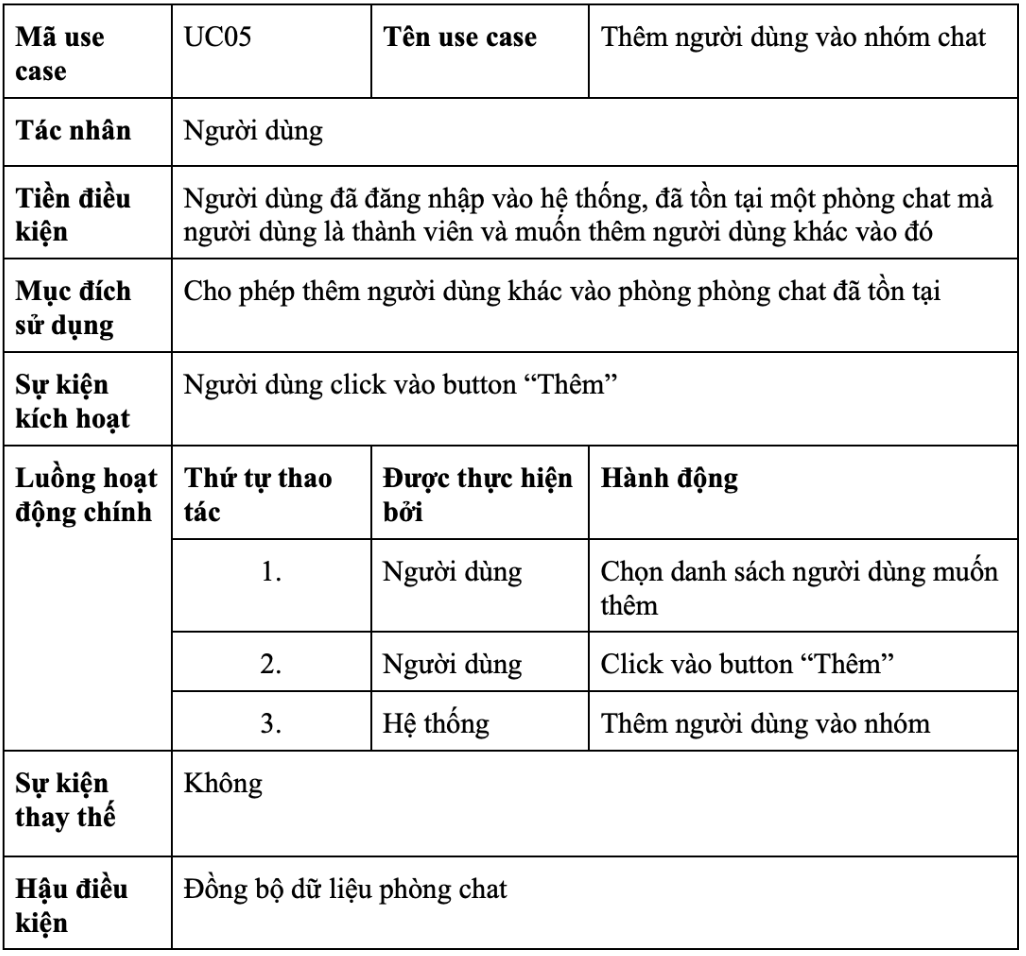
\includegraphics[width=1\linewidth]{Hinhve/UseCase/Specification/Them_Nguoi_Dung_Vao_Nhom_Chat.png}
%     \caption{Bảng đặc cả use case Thêm người dùng vào nhóm chat}
%     \label{fig:dang_xuat}
% \end{figure} 

\newpage
\subsection{Đặc cả use case Xoá người dùng khỏi phòng chat}
\begin{longtable}{
|>{\raggedright\arraybackslash}m{0.15\linewidth}
|>{\raggedright\arraybackslash}m{0.15\linewidth}
|>{\raggedright\arraybackslash}m{0.2\linewidth}
|>{\raggedright\arraybackslash}m{0.4\linewidth}|}
    \hline
    \textbf{Mã usecase} & UC06 & \textbf{Tên Use case} & {Xoá người dùng khỏi phòng chat} \\ \hline
    \textbf{Mô tả} & \multicolumn{3}{l|}{Xoá thành viên nhóm khỏi phòng chat đang tồn tại}\\ \hline
    \textbf{Tác nhân} & \multicolumn{3}{l|}{Người dùng}\\ \hline
    \textbf{Tiền điều kiện} & \multicolumn{3}{l|}{Người dùng đã đăng nhập vào hệ thống, là thành viên phòng chat} \\ \hline
    \textbf{Sự kiện kích hoạt} & \multicolumn{3}{l|}{Người dùng click thành viên và chọn “Xoá”}\\ \hline
    \textbf{Luồng sự kiện chính} & \multicolumn{3}{l|}{
    \begin{subtable}{0.8\linewidth}
        \centering
        \begin{tabular}{|>{\raggedright\arraybackslash}m{0.06\linewidth}|>{\raggedright\arraybackslash}m{0.24\linewidth}|>{\raggedright\arraybackslash}m{0.6\linewidth}|}
        \textbf{STT} & \textbf{Thực hiện} & \textbf{Hành động} \\
        \hline
        1 & Người dùng & Chọn danh sách người dùng muốn thêm \\ \hline
        2 & Người dùng & Click vào button “Thêm” \\ \hline
        3 & Hệ thống & Thêm người dùng vào nhóm \\ \hline
       \end{tabular}
    \end{subtable}
    \hfill
    }\\ \hline
     \textbf{Luồng sự kiện thay thế} & \multicolumn{3}{l|}{
    \begin{subtable}{0.8\linewidth}
        Không
    \end{subtable}
    \hfill
    } \\ \hline
     \textbf{Hậu điều kiện} & \multicolumn{3}{l|}{Đồng bộ dữ liệu phòng chat và hiển thị}\\ \hline
    \caption{Đặc tả usecase Xoá người dùng khỏi phòng chat}
    \label{table:usecaseDangNhap}
\end{longtable}



\section{Các yêu cầu phi chức năng}
\label{section:2.5}
\subsection{Yêu cầu về bảo mật}
Mật khẩu của người dùng phải được mã hoá bởi hàm băm. Các request lên server phải được đính kèm token. Tin nhắn người dùng trước khi được gửi và lưu trữ trên cơ sở dữ liệu phải được mã hoá.

Khi triển khai trên hệ thống thực tế phải sử dụng giao thức HTTPS để giao tiếp giữa server và client cho phép trao đổi thông tin một cách an toàn trên internet. 
\subsection{Yêu cầu về hiệu năng}
Thời gian phản hồi chấp nhận được. Đối với các api gửi và nhận ảnh hoặc video, thời gian phản hồi trung bình cần phải nhỏ hơn kích thước của dữ liệu tính bằng MB chia cho 1(MB/1s) được coi là chấp nhận được.
\subsection{Yêu cầu về giao diện}
Ngôn ngữ sử dụng là Tiếng Việt, giao diện thân thiện với người dùng. Hỗ trợ giao diện sáng và tối. 

Bố cục của ứng dụng: phải được thiết kế phù hợp với nhiều loại màn hình của các phiên bản iPhone. Tỷ lệ, kích thước và vị trí những phần tử hiển thị phải được sắp xếp hợp lý. 

Màu sắc: màu sắc giữa các thành phần của ứng dụng phải có sự thống nhất, sử dụng 2 màu chính là trắng và xanh nước biển.

Thiết kế nút bấm: nút bấm sử dụng các icon tượng hình. Các icon được cung cấp bởi Apple. Tất cả các icon đều tuân theo chuẩn Material Design cả về màu sắc lẫn kích thước.

Thứ tự, cấu trúc các màn hình: các màn hình phải được sắp xếp hợp lý, chỉ nên cần tối đa 3 đến 4 chạm (số lần tương tác trên màn hình giao diện) để người dùng thực hiện được mục đích của mình.

Với những màn hình hiển thị dữ liệu từ server trả về, công việc đồng bộ dữ liệu từ server phải được đưa vào luồng phụ, tránh cho giao diện bị giật và không phản hồi lại thao tác người dùng khi sử dụng.

% Chương này có độ dài từ 9 đến 11 trang.

% Với phương pháp phân tích thiết kế hướng đối tượng, sinh viên sử dụng biểu đồ use case theo hướng dẫn của template này. Với các phương pháp khác, sinh viên trao đổi với giáo viên hướng dẫn để đổi tên và sắp xếp lại đề mục cho phù hợp. Ví dụ, thay vì sử dụng biểu đồ use case, sinh viên đi theo hướng tiếp cận Agile có thể dùng User Story.

% \section{Khảo sát hiện trạng}
% \label{section:2.1}
% Thông thường, khảo sát chi tiết về hiện trạng và yêu cầu của phần mềm sẽ được lấy từ ba nguồn chính, đó là (i) người dùng/khách hàng, (ii) các hệ thống đã có, (iii) và các ứng dụng tương tự.
% Sinh viên cần tiến hành phân tích, so sánh, đánh giá chi tiết ưu nhược điểm của các sản phẩm/nghiên cứu hiện có. Sinh viên có thể lập bảng so sánh nếu cần thiết. Kết hợp với khảo sát người dùng/khách hàng (nếu có), sinh viên nêu và mô tả sơ lược các tính năng phần mềm quan trọng cần phát triển.

% \section{Tổng quan chức năng}
% \label{section:2.2}
% Phần \ref{section:2.2} này có nhiệm vụ tóm tắt các chức năng của phần mềm. Trong phần này, sinh viên lưu ý chỉ mô tả chức năng mức cao (tổng quan) mà không đặc tả chi tiết cho từng chức năng. Đặc tả chi tiết được trình bày trong phần \ref{section:2.3}.

% \subsection{Biểu đồ use case tổng quát}
% \label{subsection:2.2.1}
% Sinh viên vẽ biểu đồ use case tổng quan và giải thích các tác nhân tham gia là gì, nêu vai trò của từng tác nhân, và mô tả ngắn gọn các use case chính.

% \subsection{Biểu đồ use case phân rã XYZ}
% \label{subsection:2.2.2}
% Với mỗi use case mức cao trong biểu đồ use case tổng quan, sinh viên tạo một mục riêng như mục \ref{subsection:2.2.2} và tiến hành phân rã use case đó. Lưu ý tên use case cần phân rã trong biểu đồ use case tổng quan phải khớp với tên đề mục.

% Trong mỗi mục như vậy, sinh viên vẽ và giải thích ngắn gọn các use case phân rã.

% \subsection{Quy trình nghiệp vụ}
% \label{subsection:2.2.3}
% Nếu sản phẩm/hệ thống cần xây dựng có quy trình nghiệp vụ quan trọng/đáng chú ý, sinh viên cần mô tả và vẽ biểu đồ hoạt động minh họa quy trình nghiệp vụ đó. Sinh viên lưu ý đây không phải là luồng sự kiện của từng use case, mà là luồng hoạt động kết hợp nhiều use case để thực hiện một nghiệp vụ nào đó.

% Ví dụ, một hệ thống quản lý thư viện có quy trình nghiệp vụ mượn trả với mô tả sơ bộ như sau: Sinh viên làm thẻ mượn, sau đó sinh viên đăng ký mượn sách, thủ thư cho mượn, và cuối cùng sinh viên trả lại sách cho thư viện. Một hệ thống có thể có một vài quy trình nghiệp vụ quan trọng như vậy.
% \section{Đặc tả chức năng}
% \label{section:2.3}
% Sinh viên lựa chọn từ 4 đến 7 use case quan trọng nhất của đồ án để đặc tả chi tiết. Mỗi đặc tả bao gồm ít nhất các thông tin sau: (i) Tên use case, (ii) Luồng sự kiện (chính và phát sinh), (iii) Tiền điều kiện, và (iv) Hậu điều kiện. Sinh viên chỉ vẽ bổ sung biểu đồ hoạt động khi đặc tả use case phức tạp.
% \subsection{Đặc tả use case A}
% \hfill
% \subsection{Đặc tả use case B}
% \hfill

% \section{Yêu cầu phi chức năng}
% \label{section:2.4}
% Trong phần này, sinh viên đưa ra các yêu cầu khác nếu có, bao gồm các yêu cầu phi chức năng như hiệu năng, độ tin cậy, tính dễ dùng, tính dễ bảo trì, hoặc các yêu cầu về mặt kỹ thuật như về CSDL, công nghệ sử dụng, v.v.


%%%%%%%%%%%%%%%%%%%%%%%%%%%%%%%%%%%

\end{document}